\section{Toward an open metaverse}
For years various companies have attempted to build closed ecosystems which look now like attempts at digital society, but are more like isolated metaverse systems, or more usefully isolated digital ecosystems. This is still happening. There's every chance that when Apple make their augmented reality play this year or next they will keep their system closed off as this tends to be their business model. Theo Priestly, CEO at Metanomics \href{https://www.linkedin.com/feed/update/urn:li:activity:6977366421034967040/}{points out} that Chinese Giant Tencent are doing similar, and he cited Figure \ref{fig:tencent}; building a closed but tightly linked suite of businesses into something that looks like a metaverse. This is not what we want to discuss in this book.
\begin{figure}
  \centering
    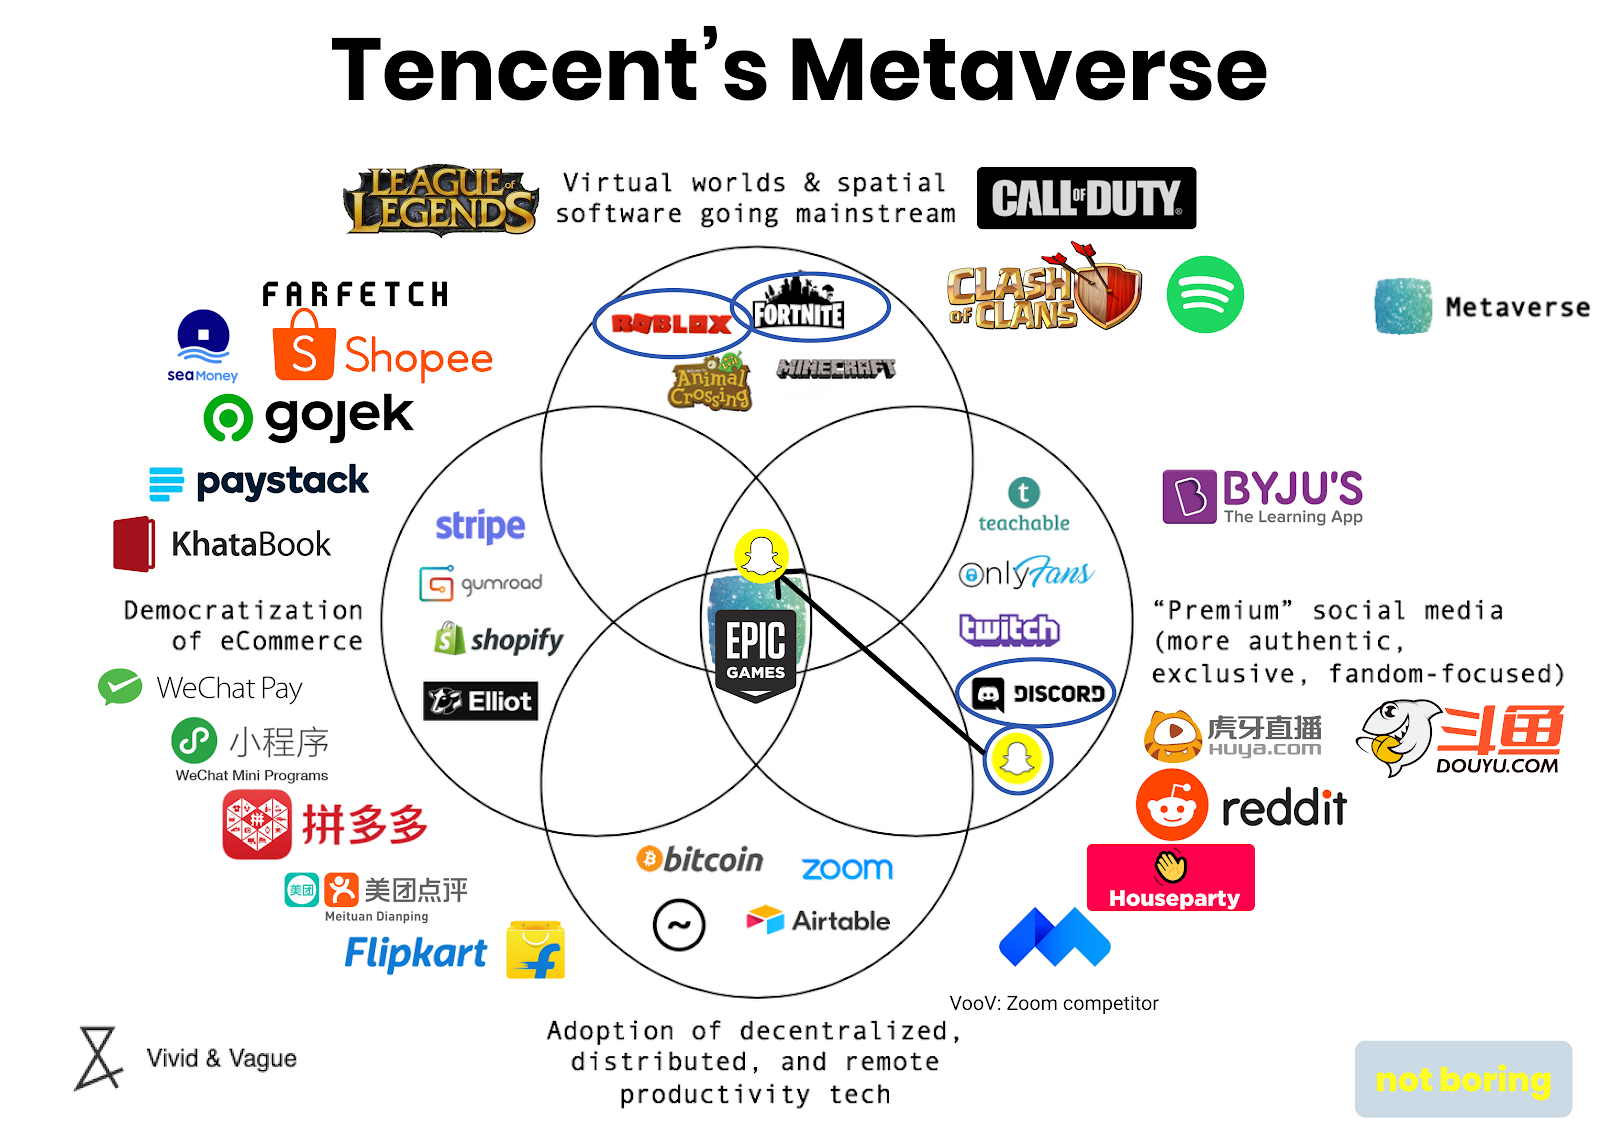
\includegraphics[width=\linewidth]{tencent}
  \caption{\href{https://www.notboring.co/p/tencents-dreams}{McCormick attempts to guess the Tencent metaverse}}
  \label{fig:tencent}
\end{figure}
For our purposes in this product design the interface between the previous chapter (NFTs) and this metaverse chapter is crucial. Punk6529 is a pseudonymous twitter account and thought leader in the ``crypto'' space. The text below encapsulates much of the reasoning that led to this book and product exploration, and is paraphrased \href{https://twitter.com/punk6529/status/1536046831045685248}{from this thread} for our purposes.\par
\textit{Bit by bit, the visualization layer of the internet will get better until it is unrecognisably better (+/- 10 years). As the visualization layer of the internet gets better, digital objects will become more useful and more important. Avatars (2D and 3D), art, schoolwork, work work, 3D virtual spaces and hundreds of other things. Not only will the objects themselves become more important, they will lead to different emergent behaviours. We see this already with avatars and mixed eponymous/pseudonymous/anonymous communities. Yes, it is the internet plumbing underneath, but just like social media changed human behaviour on the internet, metaverse type experiences will further change it. NFT Twitter + Discord + various virtual worlds is a form of early metaverse. I feel like I am entering a different world here, not just some websites. The most important question for the health of the internet/metaverse/human society in the 2030s will be decided now. And that question is: "who stores the definitive ownership records of those digital objects". There are two answers: a company's database OR a blockchain. If we end up with "a company's database" we will end up with all the web2 dysfunctions, but worse. SMTP is an open protocol that anyone can use so we don't have societal level fights on "who is allowed to use email". Short messaging online ended up becoming Twitter. So we end up having the most absurd, surreal discussions on the topic of "who is allowed to use short-messaging" being dependant on "who is the CEO of Twitter". There is no way this is the correct architecture for our progressively more digital economy.... If this is your first time around here, we are fighting for an open metaverse.''}\par
It seems that industry shares much of this opinion regarding an open metaverse. The proposal of a persistent interactive digital universe online is \textbf{so} vast that major players recognise that they will not be able to monopolise this space, though Facebook/Meta are clearly attempting to. The \href{https://metaverse-standards.org/news/press-releases/leading-standards-organizations-and-companies-unite-to-drive-open-metaverse-interoperability/}{Metaverse Standards Forum} is clearly an attempt by the other industry players to catch up and then get out ahead of Meta in this regard. It's also possible to view this as just another land grab, but through the vehicle of a standards body. Time will tell. They say:\par
\textit{``Announced today, The Metaverse Standards Forum brings together leading standards organizations and companies for industry-wide cooperation on interoperability standards needed to build the open metaverse. The Forum will explore where the lack of interoperability is holding back metaverse deployment and how the work of Standards Developing Organizations (SDOs) defining and evolving needed standards may be coordinated and accelerated. Open to any organization at no cost, the Forum will focus on pragmatic, action-based projects such as implementation prototyping, hackathons, plugfests, and open-source tooling to accelerate the testing and adoption of metaverse standards, while also developing consistent terminology and deployment guidelines.''}\par
This looks like it will be a useful project and community for the purposes outlined in this book, but the technology is young enough (in that it doesn't really exist) for multiple approaches to be trailed.\par
Europe is making metaverse a priority with \href{https://digital-strategy.ec.europa.eu/en/policies/virtual-and-augmented-reality-coalition}{The Virtual and Augmented Reality Industrial Coalition}. President von der Leyen’s State of the Union \href{https://state-of-the-union.ec.europa.eu/system/files/2022-09/SOTEU_2022_Letter_of_Intent_EN_0.pdf}{letter of intent says}:  ``We will continue looking at new digital opportunities and trends, such as the metaverse.'' 
\subsection{Primitives}
OpenAI identified the following 5 points about metaverse, in response to the query ``What are 5 key points I should know when studying metaverse?''
\begin{itemize}
\item Metaverse is a virtual reality platform that allows users to interact with each other and with digital objects in a virtual space.
\item Metaverse is a decentralized platform, meaning that there is no central authority or server that controls the platform.
\item Metaverse is an open platform, meaning that anyone can develop applications for the platform.
\item Metaverse is a secure platform, meaning that all data and transactions are encrypted and secure.
\item Metaverse is a scalable platform, meaning that it can support a large number of users and a large number of transactions.
\end{itemize}
This is an unexpectedly great answer, probably the cleanest we have found. The \href{https://metaverse-standards.org/}{Metaverse Standard Forum} highlights the following, which reads like the output from a brainstorm between academia and industry stakeholders.
\begin{itemize}
\item collaborative spatial computing
\item interactive 3D graphics 
\item augmented and virtual reality
\item photorealistic content authoring
\item geospatial systems
\item end-user content tooling
\item digital twins
\item real-time collaboration
\item physical simulation
\item online economies
\item multi-user gaming
\item new levels of scale and immersiveness. 
\end{itemize}
It's not a useless list by any means, but it lacks the kind of product focus we need for detailed exploration of value and trust transfer. \par
Mystakidis identifies the following \cite{mystakidis2022metaverse}:
\begin{itemize}
\item Principles
\begin{itemize}
\item Interoperable
\item Open
\item Hardware agnostic
\item Network
\end{itemize}
\item Technologies
\begin{itemize}
\item Virtual reality
\item Augmented reality
\item Mixed reality
\end{itemize}
\item Affordances
\begin{itemize}
\item Immersive
\item Embodiment
\item Presence
\item Identity construction
\end{itemize}
\item Challenges
\begin{itemize}
\item Physical well-being
\item Psychology
\item Ethics
\item Privacy
\end{itemize}
\end{itemize}
This is quite an academic list. A lot of these words will be explored in the next section which is more of an academic literature review.\par
Nevelsteen attempted to identify key elements for a `virtual work' in 2018 and these are relevant now, and described rigorously in the appendix of his paper \cite{nevelsteen2018virtual}:
\begin{itemize}
\item Shared Temporality, meaning that the distributed users of the virtual world share the same frame of time.
\item Real time which he defines as ``not turn based''.
\item Shared Spatiality, which he says can include an `allegory' of a space, as in text adventures. It seems this might extend to a spoken interface to a mixed reality metaverse.
\item ONE Shard is a description of the WLAN network architecture, and conforms to servers in a connected open metaverse.
\item Many human agents simply means that more than one person can be represented in the virtual world and corresponds to `social' in our description.
\item Many Software Agents corresponds to AI actors in our descriptions. Non playing characters would be the gaming equivalent.
\item Virtual Interaction pertains to any ability of a user to interact actively with the persistent virtual scene, and is pretty much a given these days.
\item Nonpausable isn't even a word, but is pretty self explanatory.
\item Persistence means that if human participants leave then the data of the virtual world continues. This applies to the scenes, the data representing actions, and objects and actors in the worlds.
\item Avatar is interesting as it might seem that having avatar representations of connected human participants is a given. In fact the shared spaces employed by Nvidia for digital engineering do not. 
\end{itemize}
Turning to industry; John Riccitiello, CEO of Unity Technologies says that metaverse is \textit{``The next generation of the internet that is:
\begin{itemize}
\item always real-time 
\item mostly 3D 
\item mostly interactive
\item mostly social
\item mostly persistent''
\end{itemize}}
Expanding this slightly we will us the following primitives of what we think are important for a metaverse:
\begin{itemize}
\item Fusing of digital and real life
\item Social first
\item Real time interactive 3d graphics first
\item Persistent
\item Supports ownership
\item Supports user generated content \cite{ondrejka2004escaping}
\item Open and extensible
\item Low friction economic actors and actions
\item Trusted / secure
%\end{itemize} 
%Added to this are externalities such as the shifting exceptions of younger demographics.
%\begin{itemize}
\item Convergence of film and games
\item Blurring of IP boundaries
\item Blurring of narrative flow
\item Multimodal and hardware agnostic
\item Mobile first experiences
\item Safeguarding, and governance
\end{itemize}
There is a \textbf{lot} of work for the creative and technical industries to do to integrate human narrative creativity this nascent metaverse, and it's not even completely clear that this is possible, or even what people want.
\section{History}
%\textbf{This chapter is being rewritten now.} %[\href{https://scholar.google.com/citations?hl=en&user=jE9vLG0AAAAJ&view_op=list_works}{Rabindra+Ratan} notes to include new researchers in the lit survey].\par
The word metaverse was coined by the author Neal Stephenson in his 1992 novel Snowcrash. It started popping up soon after in \href{https://www.newscientist.com/article/mg14819994-000-how-to-build-a-metaverse/}{news articles} and research papers \cite{mclellan1993avatars}, but in the last five years it has been finding a new life within a silicon valley narrative. Perhaps in response to this Stephenson is now working with a company called \href{https://www.lamina1.com/}{Lamina1} which actually looks a lot like the rest of this book, so perhaps we have been on the right track.\par
There were clear precursors to modern social VR, such as \href{https://www.howtogeek.com/778554/remembering-vrml-the-metaverse-of-1995/}{VRML in the 1990's} which laid much of the groundwork for 3D content over networked computers.\par% The author used to create commercial 3D scenes on Silicon Graphics systems back in the late 90s.\par
It might seem that there would be a clear path from there to now, in terms of a metaverse increasingly meaning connected social virtual spaces, but this has not happened. Instead interest in metaverse as a concept waned, MMORG (described later) filled in the utility, and then recently an entirely new definition emerged. Park and Kim surveyed dozens of different historical interpretations of the word, and the generational reboot they describe makes it even less clear \cite{park2022metaverse}. The concept of the Metaverse is extremely plastic at this time (Figure \ref{fig:muskWeb3}).\par
It's arguable that what will be expanding in this chapter is more appropriately `Cyberspace' as described by William Gibson in Neuromancer \cite{gibson2019neuromancer} \textit{``A global domain within the information environment consisting of the interdependent network of information systems infrastructures including the Internet, telecommunications networks, computer systems, and embedded processors and controllers.''}\par
Park and Kim identify the generational inflection point which has led to the resurgence of the concept of Metaverse \cite{park2022metaverse}: 
\textit{``Unlike previous studies on the Metaverse based on Second Life, the current Metaverse is based on the social value of Generation Z that online and offine selves are not different.''} \par

Brett Leonard, writer director of Lawnmower Man talks about the pressing need to get out in front of moral questions in the development of metaverse applications. He stressed that wellbeing will be a crucial underpinning of the technology because of the inherent intimacy of immersion in virtual spaces. He suggests that emotional engagement with storied characters is needed to satisfy the human need for narrative, and that this should be utopian by design to stave off the worst of dystopian emergent characteristics of the technology.\par



The book will aim to build toward an understanding of metaverse as a useful social mixed reality, that allows low friction communication and economic activity, within groups, at a global scale. Cryptography and distributed software can assist us with globally `true' persistence of digital data, so we will look to integrate this with our social XR.  This focus on persistence, value, and trust means it's most appropriate to focus on business uses as there is more opportunity for value creation which will be important to bootstrap this technology.\par
This chapter will first attempt to frame the context for telepresence (the academic term for communicating through technology), and then explain the increasingly polarised options for metaverse. It's useful to precisely identify the primitives of the product we would like to see here, so this chapter is far more a review of academic literature in the field, culminating in a proposed framework.\par
\begin{figure}
  \centering
    \includegraphics[width=\linewidth]{muskWeb3}
  \caption{Elon Musk agrees with this on Twitter. It's notable that Musk is now Twitters' \href{https://twitter.com/paraga/status/1511320953598357505}{biggest shareholder}, and has been vocal about Web2 censorship on the platform.}
  \label{fig:muskWeb3}
\end{figure}

\section{Video conferencing, the status quo}
Video-conferencing has become more popular as technology improves, as it gets better integrated with ubiquitous cloud business support suites, and as a function of the global pandemic and changing work patterns. There is obviously increasing demands for real-time communication across greater distances.\par
The full effects of video-conferencing on human communication are still being explored, as seen in the experimental \href{https://news.microsoft.com/innovation-stories/microsoft-teams-together-mode/}{``Together Mode''} within Microsoft Teams. Video-conferencing is presumed to be a somewhat richer form of communication than email and telephone, but not quite as informative as face-to-face communication. \par
In this section we look at the influence of eye contact on communication and how video-conferencing mediates both verbal and non-verbal interactions. Facilitation of eye contact is a challenge that must be addressed so that video-conferencing can approach the rich interactions of face-to-face communication. This is an even bigger problem in the emerging metaverse systems, so it's important that we examine the history and trajectory.\par
There is a tension emerging for companies who do not necessarily need to employ remote meeting technology, but also cannot afford to ignore the competitive advantages that such systems bring. In an experiment preformed well before the 2020 global pandemic at CTrip, Bloom et al describe how home working led to a 13\% performance increase, of which about 9\% was from working more minutes per shift (fewer breaks and sick-days) and 4\% from more calls per minute (attributed to a quieter working environment) \cite{Bloom2015}. Home workers also reported improved work satisfaction and experienced less turnover, but their promotion rate conditional on performance fell. This speaks to a lack of management capability with such systemic change. It's clearly a complex and still barely understood change within business and management. \par
Due to the success of the experiment, CTrip rolled-out the option to work from home to the whole company, and allowed the experimental employees to re-select between the home or office. Interestingly, over half of them switched, which led to the gains almost doubling to 22\%. This highlights the benefits of learning and selection effects when adopting modern management practices like working from home. Increasingly this is becoming a choice issue for prospective employees, and an advantage for hiring managers to be able to offer it.\par
More recent research by Barrero, Bloom and Davies found that working from home is likely to be ``sticky'' \cite{barrero2021working}. They found:
\begin{itemize}
\item better-than-expected WFH experiences, 
\item new investments in physical and human capital that enable WFH, 
\item greatly diminished stigma associated with WFH, 
\item lingering concerns about crowds and contagion risks,
\item a pandemic-driven surge in technological innovations that support WFH.
\end{itemize}
More recently Enterprise Collaboration Systems (ECS) provide rich document management, sharing, and collaboration functionality across an organisation. The enterprise ECS system may integrate collaborative video \cite{prakash2020characteristic}. This is for instance the case with Microsoft Teams / Sharepoint. This integration of ECS should be considered when thinking about social VR systems which wish to support business, value, and trust. It is very much the case that large technology providers are attempting to integrate their `business back end' systems into their emerging metaverse systems. Open source equivalents are currently lacking.
\subsection{Pandemic drives adoption}
The ongoing global COVID-19 pandemic is \href{https://blog.yelp.com/news/the-future-of-work-is-remote/}{changing how people work}, toward a new global `normal'. Some ways of working are overdue transformation, and will be naturally disrupted. In the UK at least it seems that there may be real appetite to shift away from old practises. This upheaval will inevitably present both challenges and opportunities.\par
Highly technical workforces, especially, can \href{https://globalworkplaceanalytics.com/telecommuting-statistics}{operate from anywhere}. The post pandemic world seems to have stronger national border controls, with a resultant shortage of highly technical staff. This has forced the hand of global business toward \href{https://www.lifeatspotify.com/being-here/work-from-anywhere}{internationally distributed teams}. \par
If only a small percentage of companies allow the option of remote working, then they gain a structural advantage, enjoying benefits of reduced travel, lower workplace infection risk across all disease, and global agility for the personnel. Building and estate costs will certainly be reduced. More diversity may be possible. Issues such as sexual harassment and bullying may be reduced.  With reduced overheads product quality may increase. If customers are happier with their services, then over time this `push' may mean an enormous shift away from centralised working practises toward distributed working. \par
Technologies which support this working style were still in their infancy at the beginning of the pandemic. The rush to `Zoom', a previously relatively unknown and insecure \cite{aiken2020zooming} web meeting product, shows how naive businesses were in this space. \par
Connection of multiple users is now far better supported, with Zoom and \href{https://www.microsoft.com/en-us/Investor/earnings/FY-2021-Q1/press-release-webcast}{Mircosoft Teams} alone supporting hundreds of millions of chats a day. This is a 20x increase on market leader Skype's 2013 figure of \href{https://www.microsoft.com/en-us/Investor/earnings/FY-2013-Q1/press-release-webcast}{280 million} connections per month. Such technologies extend traditional telephony to provide important multi sensory cues.  However, these technologies demonstrate shortfalls compared to a live face-to-face meeting, which is generally agreed to be optimal for human-human interaction \cite{Wolff2008}.\par
While the research community and business are learning how to adapt working practises to web based telepresence \cite{oeppen2020human}, there remains little technology support for ad-hoc serendipitous meetings between small groups. It's possible that Metaverse applications can help to fill this gap, by gamification of social spaces, but the under discussed problems with video conferencing are likely to be even worse in such systems. \par
Chris Herd of ``FirstBase'' (who admittedly have a bias) provides some fascinating speculations: \par
\textit{``I've spoken to 2,000+ companies with 40M+ employees about remote work in the last 12 months 
A few predictions of what will happen before 2030:
\begin{itemize}
\item Rural Living: World-class people will move to smaller cities, have a lower cost of living \& higher quality of life.
\item These regions must innovate quickly to attract that wealth. Better schools, faster internet connections are a must.
\item Async Work: Offices are instantaneous gratification distraction factories where synchronous work makes it impossible to get stuff done.
\item Tools that enable asynchronous work are the most important thing globally remote teams need. A lot of startups will try to tackle this.
\item Hobbie Renaissance: Remote working will lead to a rise in people participating in hobbies and activities which link them to people in their local community.
\item This will lead to deeper, more meaningful relationships which overcome societal issues of loneliness and isolation.
\item Diversity \& Inclusion: The most diverse and inclusive teams in history will emerge rapidly
Companies who embrace it have a first-mover advantage to attract great talent globally. Companies who don't will lose their best people to their biggest competitors.
\item Output Focus: Time will be replaced as the main KPI for judging performance by productivity and output.
\item Great workers will be the ones who deliver what they promise consistently
\item Advancement decisions will be decided by capability rather than who you drink beer with after work.
\item Private Equity: The hottest trend of the next decade for private equity will see them purchase companies, make them remote-first
The cost saving in real-estate at scale will be eye-watering. The productivity gains will be the final nail in the coffin for the office
Working Too Much: Companies worry that the workers won't work enough when operating remotely.
\item The opposite will be true and become a big problem.
\item Remote workers burning out because they work too much will have to be addressed.
\item Remote Retreats: Purpose-built destinations that allow for entire companies to fly into a campus for a synchronous week.
\item Likely staffed with facilitators and educators who train staff on how to maximize effectiveness.
\item Life-Work Balance: The rise of remote will lead to people re-prioritizing what is important to them.
\item Organizing your work around your life will be the first noticeable switch. People realizing they are more than their job will lead to deeper purpose in other areas.
\item Bullshit Tasks: The need to pad out your 8 hour day will evaporate, replaced by clear tasks and responsibilities.
\item Workers will do what needs to be done rather than wasting their trying to look busy with the rest of the office
\end{itemize}
''}

            \subsection{Point to Point Video Conferencing}
                O'Malley et al. showed that face-to-face and video mediated employed  visual cues for mutual understanding, and that addition of video to the audio channel aided confidence and mutual understanding. However, video mediated did not provide the clear cues of being co-located \cite{OMalley1996}.\par
                Dourish et al. make a case for not using face-to-face as a baseline for comparison, but rather that analysis of the efficacy of remote tele-collaboration tools should be made in a wider context of connected multimedia tools and `emergent communicative practises' \cite{Dourish1996}. While this is an interesting viewpoint it does not necessarily map well to a recreation of the ad-hoc meeting.\par
There is established literature on human sensitivity to eye contact in both 2D and 3D VC \cite{Criminisi2003, Van_Eijk2010}, with an accepted minimum of 5-10 degrees before observers can reliably sense they are not being looked at \cite{Chen2002}. Roberts et al. suggested that at the limit of social gaze distance (~4m) the maximum angular separation between people standing shoulder to shoulder in the real world would be around 4 degrees\cite{Roberts2013}. \par
                Sellen found limited impact on turn passing when adding a visual channel to audio between two people when using Hydra, an early system which provided multiple video conference displays in an intuitive spatial distribution\cite{Sellen1992}. She did however, find that the design of the video system affected the ability to hold multi-party conversations \cite{Sellen1995}.\par
                Monk and Gale describe in detail experiments which they used 
 for examining gaze awareness in communication which is mediated and unmediated by technology.  
  They   found that gaze awareness increased message understanding  
  \cite{Monk2002}.\par
                Both Kuster et al. and Gemmel et al. have successfuly demonstrated software systems which can adjust eye gaze to correct for off axis capture in real time video systems\cite{Gemmell2000, Kuster2012}.\par
                Shahid et al. conducted a study on pairs of children playing games with and without video mediation and concluded that the availability of mutual gaze affordance enriched social presence and fun, while its absence dramatically affects the quality of the interaction. They used the `Networked Minds', a social presence questionnaire.                
        \subsection{Triadic and Small Group}
Early enthusiasm in the 1970's for video conferencing, as a medium for small group interaction quickly turned to disillusionment. It was agreed after a flurry of initial research that the systems at the time offered no particular advantage over audio only communication, and at considerable cost \cite{Williams1977}.\par
Something in the breakdown of normal visual cues seems to impact the ability of the technology to support flowing group interaction. Nonetheless, some non-verbal communication is supported in VC with limited success. \par
Additional screens and cameras can partially overcome the limitation of no multi-party support (that of addressing a room full of people on a single screen) by making available more bidirectional channels. For instance, every remote user can be a head on a screen with a corresponding camera. The positioning of the screens must then necessarily match the physical organization of the remote room.\par
Egido provides an early review of the failure of VC for group activity, with the ``misrepresentation of the technology as a substitute for face-to-face" still being valid today \cite{Edigo1988}.\par
Commercial systems such as Cisco Telepresence Rooms cluster their cameras above the centre screen of three for meetings using their telecollaboration product, while admitting that this only works well for the central seat of the three screens. They also group multiple people on a single screen in what Workhoven et al. dub a ``non-isotropic" configuration \cite{Pejsa2016}. They maintain that this is a suitable trade off as the focus of the meeting is more generally toward the important contributor in the central seat. This does not necessarily follow for less formal meeting paradigms.\par
            In small groups, it is more difficult to align non-verbal cues between all  parties, and at the same time, it is more important because the hand-offs between parties are more numerous and important in groups. A breakdown in conversational flow in such circumstances is harder to solve. A perception of the next person to talk must be resolved for all parties and agreed upon to some extent.\par
                However, most of the conventional single camera, and expensive multi camera VC systems, suffer a fundamental limitation in that the offset between the camera sight lines and the lines of actual sight introduce incongruities that the brain must compensate for \cite{Wolff2008}.\par
   %  For experimental design Bailenson found the game `20 questions' to be effective in analysis of triadic attention, specifically watching the head gaze \cite{Bailenson2002}.
\subsection{Other Systems to Support Business}                  
There have been many attempts to support group working and rich data sharing between dispersed groups in a business setting. So called 'smart spaces' allow interaction with different displays for different activities and add in some ability to communicate with remote or even mobile collaborators on shared documents \cite{Bardram2012}, with additional challenges for multi-disciplinary groups who are perhaps less familiar with one or more of the technology barriers involved \cite{Adamczyk2007}.\par
Early systems like clearboard \cite{Ishii1993} demonstrated the potential for smart whiteboards with a webcam component for peer-to-peer collaborative working. Indeed it is possible to support this modality with Skype and a smartboard system (and up to deployments such as Accessgrid). They remain relatively unpopular however.\par
\subsection{Mona Lisa Type Effects}
Almost all traditional group video meeting tools suffer from the so-called Mona Lisa effect which describes the phenomenon where the apparent gaze of a portrait or 2 dimensional image always appears to look at the observer regardless of the observer's position \cite{Vishwanath2005, Anstis1969, Wollaston1824}. This situation manifests when the painted or imaged subject is looking into the camera or at the eyes of the painter \cite{Loomis2008, Fullwood2006}.\par
Single user-to-user systems based around bidirectional video implicitly align the user's gaze by constraining the camera to roughly the same location as the display. When viewed away from this ideal axis, it creates the feeling of being looked at regardless of where this observer is \cite{Moubayed2012, Vishwanath2005, Anstis1969, Wollaston1824}, or the ``collapsed view effect'' \cite{Nguyen2005} where perception of gaze transmitted from a 2 dimensional image or video is dependent on the incidence of originating gaze to the transmission medium. \par
Multiple individuals using one such channel can feel as if they are being looked at simultaneously, leading to a breakdown in the normal non-verbal communication which mediates turn passing \cite{Vertegaal2002}.    
There is research investigating this sensitivity when the gaze is mediated by a technology, finding that ``disparity between the optical axis of the camera and the looking direction of a looker should be at most 1.2 degrees in the horizontal direction, and 1.7 degrees in vertical direction to support eye contact" \cite{Van_Eijk2010, Bock2008}. It seems that humans assume that they are being looked at unless they are sure that they are not \cite{Chen2002}.\par
To be clear, there are technological solutions to this problem, but it's useful in the context of discussing metaverse to know that this problem exists. It's known that there are cognitive dissonances around panes of video conference images, but it seems that the effect is truely limited to 2D surfaces. A 3D projection surface (a physical model of a human) designed to address this problem completely removed the Mona Lisa effect \cite{Moubayed2012}.\par 
Metaverse then perhaps offers the promise of solving this, making more natural interaction possible, but it's clearly a long way from delivering on those promises right now. We need to understand what's important and try to map these into a metaverse product.
\section{What's important for human communication}
\subsection{Vocal}
The ubiquitous technology to mediate conversation is, of course, the telephone. The \href{https://www.ericsson.com/en/reports-and-papers/mobility-report/reports/november-2021}{2021 Ericsson mobility report}  states that there are around 8 billion mobile subscriptions globally. More people have access to mobile phones than to working toilets \href{https://www.unicef.org/innovation/stories/more-cellphones-toilets}{according to UNICEF}.\par
Joupii and Pan designed a system which focused attention on spatially correct high definition audio. They found ``significant improvement over traditional audio conferencing technology, primarily due to the increased dynamic range and directionality. \cite{Jouppi2002}. Aoki et al. also describe an audio only system with support for spatial cues \cite{Aoki2003}.\par
In the following sections we will attempt to rigorously identify just what is important for our proposed application of business centric communication, supportive of trust, and thereby value transfer.\par
In his book `Bodily Communication' \cite{Argyle1988} Michael Argyle divides vocal signals into the following categories:
\begin{enumerate}
\item Verbal
\item Non-Verbal Vocalisations
\begin{enumerate}
       \item Linked to Speech
       \begin{enumerate}
         \item   Prosodic
         \item   Synchronising
         \item   Speech Disturbances
         \end{enumerate}
      \item  Independent of Speech
      \begin{enumerate}
        \item    Emotional Noises
         \item   Paralinguistic (emotion and interpersonal attitudes)
         \item   Personal voice and quality of accent
         \end{enumerate}
\end{enumerate}
\end{enumerate}               
Additional to the semantic content of verbal communication there is a rich layer of meaning in pauses, gaps, and overlaps \cite{Heldner2010} which help to mediate who is speaking and who is listening in multi-party conversation. This mediation of turn passing, to facilitate flow, is by no means a given and is highly dependent on context and other factors \cite{Kleinke1986}. Interruptions are also a major factor in turn passing.\par
This extra-verbal content \cite{Ting-Toomey2012} extends into physical cues, so-called `nonverbal' cues, and there are utterances which link the verbal and non-verbal \cite{Otsuka2005}. This will be discussed later, but to an extent, it is impossible to discuss verbal communication without regard to the implicit support which exists around the words themselves.\par
In the context of all technology-mediated conversation the extra-verbal is easily compromised if technology used to support communication over a distance does not convey the information, or conveys it badly. This can introduce additional complexity \cite{Otsuka2005}.\par
These support structures are pretty much lacking in metaverse XR systems. The goal then here perhaps is to examine the state-of-the-art, and remove as many of the known barriers as possible. Such a process might better support trust, which might better support the kind of economic and activity we seek to engineer.\par
When examining just verbal / audio communication technology it can be assumed that the physical non-verbal cues are lost, though not necessarily unused. In the absence of non-verbal cues it falls to timely vocal signals to take up the slack when framing and organising the turn passing. For the synchronising of vocal signals between the parties to be effective the systemic delays must remain small. System latency, the inherent delays added by the communication technology, can allow slips or a complete breakdown of 'flow' \cite{katagiri2007aiduti}. This problem can be felt in current social VR platforms, though people don't necessarily identify the cause of the breakdown correctly. In the main they feel to the users like a bad ``audio-only'' teleconference.\par
With that said, the transmission of verbal / audio remains the most critical element for interpersonal communication as the most essential meaning is encoded semantically. There is a debate about ratios of how much information is conveyed through the various human channels \cite{Loomis2012}, but it is reasonable to infer from its ubiquity that support for audio is essential for meaningful communication over a distance. We have seen that it must be timely, to prevent a breakdown of framing, and preferably have sufficient fidelity to convey sub-vocal utterances. \par
For social immersive VR for business users, a real-time network such as websockets, RTP, or UDP seems essential, much better microphones are important, and the system should support both angular spatialisation, and respond to distance between interlocutors.
\subsection{Nonverbal}
We have already seen that verbal exchanges take place in a wider context of sub vocal and physical cues. In addition, the spatial relationship between the parties, their focus of attention, their gestures and actions, and the wider context of their environment all play a part in communication \cite{Goodwin2000}. These are identified as follows by Gillies and Slater \cite{Gillies2005} in their paper on virtual agents.\par
\begin{itemize}
\item Posture and gesture
\item Facial expression
\item Gaze
\item Proxemics
\item Head position and orientation
\item Interactional synchrony
\end{itemize}

This is clearly important for our proposed metaverse application. Below we will examine these six areas by looking across the wider available research.

\subsubsection{Gaze}
Of particular importance is judgement of eye gaze which is normally fast, accurate and automatic, operating at multiple levels of cognition through multiple cues \cite{Argyle1988,Argyle1976,Argyle1965,Argyle1976,Argyle1969, Kendon1967,Monk2002}.\par
Gaze in particular aids smooth turn passing \cite{Hedge1978} \cite{Novick1996} and lack of support for eye gaze has been found to decrease the efficiency of turn passing by 25\% \cite{Vertegaal2000}.\par
There are clear patterns to eye gaze in groups, with the person talking, or being talked to, probably also being looked at \cite{Vertegaal2001} \cite{Langton2000}. To facilitate this groups will tend to position themselves to maximally enable observation of the gaze of the other parties \cite{Kendon1967}. This intersects with proxemics which will be discussed shortly.  In general people look most when they are listening, with short glances of 3-10 seconds \cite{Argyle1965}. %Novick et al. performed analysis gaze patterns utilised for on task hand-off, which is potentially useful for extension into shared task experiment design \cite{Novick1996}.\par
Colburn et al. suggest that gaze direction and the perception of the gaze of others directly impacts social cognition \cite{Colburn2000} and this has been supported in a follow up study \cite{Macrae2002}.\par
The importance of gaze is clearly so significant in evolutionary terms that human acuity for eye direction is considered high at ~30 sec arc \cite{Symons2004} with straight binocular gaze judged more accurately than straight monocular gaze \cite{Kluttz2009}, when using stereo vision. \par
Regarding the judgement of the gaze of others, Symons et al. suggested that ``people are remarkably sensitive to shifts in a person's eye gaze'' in triadic conversation \cite{Symons2004}. 
This perception of the gaze of others operates at a low level and is automatic. Langton et al. cite research stating that the gaze of others is ``able to trigger reflexive shifts of an observer's visual attention'' and further discuss the deep biological underpinnings of gaze processing \cite{Langton2000}. \par  
When discussing technology-mediated systems, Vertegaal \& Ding suggested that understanding the effects of gaze on triadic conversation is ``crucial for the design of teleconferencing systems and collaborative virtual environments'' \cite{Vertegaal2002}, and further found correlation between the amount of gaze, and amount of speech. Vertegaal \& Slagter suggest that ``gaze function(s) as an indicator of conversational attention in multiparty conversations'' \cite{Vertegaal2001}. It seems like is we are to have useful markets within social immersive environments then support for natural gaze effects should be a priority.\par  
Wilson et al. found that subjects can ``discriminate gaze focused on adjacent faces up to [3.5m]'' \cite{Wilson2000}. This perhaps gives us a testable benchmark within a metaverse application which is eye gaze enabled. In this regard Schrammel et al. investigated to what extent embodied agents can elicit the same responses in eye gaze detection \cite{Schrammel2007}.\par       
Vertegaal et al. found that task performace was 46\% better when gaze was synchronised in their telepresence scenario. As they point out, gaze synchonisation (temporal and spatial) is `commendable' in all such group situations, but the precise utility will depend upon the task \cite{Vertegaal2002}.\par
There has been some success in the automatic detection of the focus of attention of participants in multi party meetings \cite{Stiefelhagen2001, Stiefelhagen2002}.  More recently, eye tracking technologies allow the recording and replaying of accurate eye gaze information \cite{Steptoe2009} alongside information about pupil dilation toward determination of honesty and social presence \cite{Steptoe2010}. It seems there are trust and honesty issues conflated with how collaborants in a virtual space are represented.\par               
In summary, gaze awareness does not just mediate verbal communication but rather is a complex channel of communication in its own right. Importantly, gaze has a controlling impact on those who are involved in the communication at any one time, including and excluding even beyond the current participants. Perhaps the systems we propose in this book need to demand eye gaze support, but it is clear that it should be recommended, and that the software selected should support the technology integration in principle.\par
\subsubsection{Mutual Gaze}
Aygyle and Cook established early work around gaze and mutual gaze, with their seminal book of the same title \cite{Argyle1976}, additionally detailing confounding factors around limitations and inaccuracies in observance of gaze and how this varies with distance \cite{Argyle1969, Argyle1988, Cook1977}.\par
Mutual gaze is considered to be the most sophisticated form of gaze awareness with significant impact on dyadic conversation especially \cite{Cook1977, Kleinke1986, Fagel2010}. The effects seem more profound than just helping to mediate flow and attention, with mutual eye gaze aiding in memory recall and the formation of impressions \cite{Bohannon2013}.\par
While reconnection of mutual eye gaze through a technology boundary does not seem completely necessary it is potentially important, with impact on subtle elements of one-to-one communication, and therefore discrimination of eye gaze direction should be bi-directional if possible, and if possible have sufficient accuracy to judge direct eye contact. In their review Bohannon et al. said that the issue of rejoining eye contact must be addressed in order to fully realise the richness of simulating face-to-face encounters \cite{Bohannon2013}.\par
Mutual gaze is a challenging affordance as bi-directional connection of gaze is not a trivial problem. It's perhaps best to view this as at the `edge' of our requirements for a metaverse.
                   \subsubsection{Mutual Gaze in Telepresence}
          We have seen that transmission of attention can broadly impact communication in subtle ways, impacting empathy, trust, cognition, and co-working patterns. Mutual gaze (looking into one another's eyes), is currently the high water mark for technology-mediated conversation.\par
          Many attempts have been made to re-unite mutual eye gaze when using tele-conferencing systems. In their 2015 review of approaches Regenbrecht and Langlotz found that none of the methods they examined were completely ideal \cite{Regenbrecht2015}. They found most promise in 2D and 3D interpolation techniques, which will be discussed in detail later, but they opined that such systems were very much ongoing research and lacked sufficient optimisation.\par
          A popular approach uses the so called 'Peppers Ghost' phenomenon \cite{Steinmeyer2013}, where a semi silvered mirror presents an image to the eye of the observer, but allows a camera to view through from behind the angled mirror surface. The earliest example of this is Rosental's two way television system in 1947 \cite{Rosenthal1947}, though Buxton et al. `Reciprocal Video Tunnel' from 1992 is more often cited \cite{Buxton1992}. This optical characteristic isn't supported by retroreflective projection technology, and besides requires careful control of light levels either side of the semi-silvered surface.\par  
The early GAZE-2 system (which makes use of Pepper's ghost) is novel in that it uses an eye tracker to select the correct camera from several trained on the remote user. This ensures that the correct returned gaze (within the ability of the system) is returned to the correct user on the other end of the network \cite{Vertegaal2003}.
Mutual gaze capability is later highlighted as an affordance supported or unsupported by key research and commercial systems.                           


\subsubsection{Head Orientation}
Orientation of the head (judged by the breaking of bilateral symmetry and alignment of nose) is a key factor when judging attention. Perception of head orientation can be judged to within a couple of degrees \cite{Wilson2000}.\par
It has been established that head gaze can be detected all the way out to the extremis of peripheral vision, with accurate eye gaze assessment only achievable in central vision \cite{Loomis2008}. This is less of use for our metaverses at this time, because user field of view is almost always restricted in such systems. More usefully, features of illumination can alter the apparent orientation of the head \cite{Troje1998}.\par
Head motion over head orientation is a more nuanced propostion and can be considered a micro gesture \cite{Boker2011}. Head tracking systems within head mounted displays can certainly detect these tiny movements, but it's clear that not all of this resolution is passed into shared virtual settings through avatars. It would be beneficial to be able to fine tune this feature within any software selected.\par
                    It is possible that 3D displays are better suited to perception of head gaze since it is suggested that they are more suitable for ``shape understanding tasks'' \cite{St_John2001}\par
                    Bailenson, Baell, and Blascovich found that giving avatars rendered head movements in a shared virtual environment decreased the amount of talking, possibly as the extra channel of head gaze was opened up. They also reported that subjectively, communication was enhanced \cite{Bailenson2002}. \par
                    Clearly head orientation is an important indicator of the direction of attention of members of a group and can be discerned even in peripheral vision. This allows the focus of several parties to be followed simultaneously and is an important affordance to replicate on any multi-party communication system. \par
\subsubsection{Combined Head and Eye Gaze}
Rienks et al. found that head orientation alone does not provide a reliable cue for identification of the speaker in a multiparty setting \cite{Rienks2010}. Stiefelhagen \& Zhu found ``that head orientation contributes 68.9\% to the overall gaze direction on average'' \cite{Stiefelhagen2002}, though head and eye gaze seem to be judged interdependently \cite{Kluttz2009}. Langton noted that head and eye gaze are ``mutually influential in the analysis of social attention'' \cite{Langton2000}, and it is clear that transmission of `head gaze' by any mediating system, enhances rather than replaces timely detection of subtle cues. Combined head and eye gaze give the best of both worlds and extend the lateral field of view in which attention can be reliably conveyed to others \cite{Loomis2008}.
\subsubsection{Other Upper Body: Overview}
While it is well evidenced that there are advantages to accurate connection of the gaze between conversational partners \cite{Argyle1969, Kleinke1986}, there is also a body of evidence that physical communication channels extend beyond the face \cite{Kleinke1986, Nguyen2009} and include both micro (shrugs, hands and arms), and macro movement of the upper body \cite{Ekman1993}. Goldin-Meadow suggests that gesturing aids conversational flow by resolving mismatches and aiding cognition \cite{Goldin-Meadow1999}.\par
                    In their technology-mediated experiment which compared face to upper body and face on a flat screen, Nguyen and Canny found that ``upper-body framing improves empathy measures and gives results not significantly different from face-to-face under several empathy measures'' \cite{Nguyen2009}. 
                    
The upper body can be broken up as follows:\par
\textbf{Facial}\\Much emotional context can be described by facial expression (display) alone \cite{Ekman1993, Chovil1991}, with smooth transition between expressions seemingly important \cite{schiano2004}. This suggests that mediating technologies should support high temporal resolution, or at least that there is a minimum resolution between which transitions between expressions become too 'categorical'. Some aspects of conversational flow appear to be mediated in part by facial expression \cite{ohba1998}. There are gender differences in the perception of facial affect \cite{Hofmann2006}.\par
\textbf{Gesturing} \\(such as pointing at objects) paves the way for more complex channels of human communication and is a basic and ubiquitous channel \cite{Iverson2005}.  Conversational hand gestures provide a powerful additional augmentation to verbal content \cite{Krauss1996}.\par
\textbf{Posture} \\Some emotions can be conveyed through upper body configurations alone. Argyle details some of these \cite{Argyle1988} and makes reference to the posture of the body and the arrangement of the arms (i.e. folded across the chest). These are clearly important cues. Kleinsmith and Bianchi-Berthouze assert that "some affective expressions may be better communicated by the body than the face" \cite{Kleinsmith2013}.\par
\textbf{Body Torque} \\In multi-party conversation, body torque, that is the rotation of the trunk from front facing, can convey aspects of attention and focus \cite{Schegloff1998}.\par
In summary, visual cues which manifest on the upper body and face can convey meaning, mediate conversation, direct attention, and augment verbal utterances. \par
\subsubsection{Effect of Shared Objects on Gaze}
Ou et al. detail shared task eye gaze behaviour ``in which helpers seek visual evidence for workers' understanding when they lack confidence of that understanding, either from a shared, or common vocabulary'' \cite{Ou2005}.\par 
  Murray et al. found that in virtual environments, eye gaze is crucial for discerning what a subject is looking at \cite{Murray2009}. This work is shown in Figure \ref{fig:murrayeyegaze}.\par
It is established that conversation around a shared object or task, especially a complex one, mitigates gaze between parties \cite{Argyle1976} and this suggests that in some situations around shared tasks in metaverses it may be appropriate to reduce fidelity of representation of the avatars. \par
\begin{figure}[!h]
\includegraphics[width=\linewidth]{murrayeyegaze.jpg}
\caption{Eye tracked eye gaze awareness in VR. Murray et al. used immersive and semi immersive systems alongside eye trackers to examine the ability of two avatars to detect the gaze awareness of a similarly immersed collaborator.}
\label{fig:murrayeyegaze}
\end{figure}                                       

  \subsubsection{Tabletop and Shared Task}
In early telepresence research Buxton and William argued through examples that ``effective telepresence depends on quality sharing of both person and task space \cite{Buxton1992}.\par
In their triadic shared virtual workspace Tang et al. found difficulty in reading shared text using a `round the table' configuration, a marked preference for working collaboratively on the same side of the table. They also found additional confusion as to the identity of remote participants \cite{Tang2010}.
Tse et al. found that pairs can work well over a shared digital tabletop, successfully overcoming a single user interface to interleave tasks \cite{Tse2007}.\par
Tang et al. demonstrate that collaborators engage and disengage around a group activity through several distinct, recognizable mechanisms with unique characteristics \cite{Tang2006}. They state that tabletop interfaces should offer a variety of tools to facilitate this fluidity.\par
Camblend is a shared workspace with panoramic high resolution video. It maintains some spatial cues between locations by keeping a shared object in the video feeds \cite{Norris2013, Norris2012}. Participants successfully resolved co-orientation within the system.\par
The t-room system implemented by Luff et al. surrounds co-located participants standing at a shared digital table with life sized body and head video representations of remote collaborators \cite{Luff2011} but found that there were incongruities in the spatial and temporal matching between the collaborators which broke the flow of conversation.
Tuddenham et al. found that co-located collaborators naturally devolved 'territory' of working when sharing a task space, and that this did not happen the same way with a tele-present collaborator \cite{Tuddenham2009}. Instead remote collaboration adapted to use a patchwork of ownership of a shared task. It seems obvious to say that task ownership is a function of working space, but it is interesting that the research found no measurable difference in performance when the patchwork coping strategy was employed.\par
The nature of a shared collaborative task and/or interface directly impacts the style of interaction between collaborators. This will have a bearing on the choice of task for experimentation \cite{Jamil2011, Jetter2011}.

\section{Psychology of Technology-Mediated Interaction}       
\subsection{Proxemics}
Proxemics is the formal study of the regions of interpersonal space begun in the late 50's by Hall and Sommers and building toward The Hidden Dimension \cite{Hall1969}, which details bands of space (Figure \ref{fig:proxemics}) that are implicitly and instinctively created by humans and which have a direct bearing on communication.
\begin{figure}[!h]
\includegraphics[width=\linewidth]{proxemics}
\caption{Bands of social space around a person Image CC0 \href{https://en.wikipedia.org/wiki/Proxemics}{from wikipedia}.}
\label{fig:proxemics}
\end{figure}                                       
Distance between conversational partners, and affiliation, also have a bearing on the level of eye contact \cite{Argyle1965} with a natural distance equilibrium being established and developed throughout, through both eye contact and a variety of subtle factors. Argyle \& Ingham provide levels of expected gaze and mutual gaze against distance \cite{Argyle1969}. These boundaries are altered by ethnicity \cite{Watson1966, Argyle1988} and somewhat by gender \cite{Bruno2013}, and age \cite{Slessor2008, Hofmann2006}.\par
Even with significant abstraction by communication systems (such as SecondLife) social norms around personal space persist \cite{Yee2007, Bailenson2001, Bailenson2003}. Bailenson \& Blascovich found that even in Immersive Collaborative Virtual Environments (ICVE's) ``participants respected personal space of the humanoid representation''\cite{Bailenson2001} implying that this is a deeply held 'low-level' psychophysical reaction \cite{Blascovich2002}. The degree to which this applies to non-humanoid avatars seems under explored.\par
Maeda et al. \cite{Maeda2004} found that seating position impacts the level of engagement in teleconferencing. Taken together with the potential for reconfiguration within the group as well as perhaps signalling for the attention of participants outside of the confines of the group in an open business metaverse setting.\par
When considering the attention of engaging with people outside the confines of a meeting Hager et al. found that gross expressions can be resolved by humans over long distances \cite{Hager1979, Argyle1988}. It seems that social interaction begins around 7.5m in the so-called `public space' \cite{Hall1969}. Recreating this affordance in a metaverse would be a function of the display resolution, and seems another `stretch goal' rather than a core requirement.\par                
\subsection{Attention}
The study of attention is a discrete branch of psychology. It is the study of cognitive selection toward a subjective or objective sub focus, to the relative exclusion of other stimulae. It has been defined as ``a range of neural operations that selectively enhance processing of information'' \cite{Carlston2013}. In the context of interpersonal communication it can be refined to apply to selectively favouring a conversational agent or object or task above other stimuli in the contextual frame.\par
Humans can readily determine the focus of attention of others in their space \cite{Stiefelhagen2001} and preservation of the spatial cues which support this are important for technology-mediated communication \cite{Sellen1992} \cite{Stiefelhagen2002}.\par
The interplay between conversational partners, especially the reciprocal perception of attention, is dubbed the perceptual crossing \cite{Deckers2013, Gibson1963}.\par
This is a complex field of study with gender, age, and ethnicity all impacting the behaviour of interpersonal attention \cite{Bente1998, Slessor2008, Argyle1988, Hofmann2006, Pan2008}.
Vertegaal has done a great deal of work on awareness and attention in technology-mediated situations and the work of his group is cited throughout this chapter \cite{Vertegaal1997}. As an example it is still such a challenge to ``get'' attention through mediated channels of communication, that some research \cite{Fels2000, Sellen1992} and many commercial systems such as `blackboard collaborate', Zoom, and Teams use tell tale signals (such as a microphone icon) to indicate when a participant is actively contributing. Some are automatic, but many are still manual, requiring that a user effectively hold up a virtual hand to signal their wish to communicate.\par
Langton et al. cite research stating that the gaze of others is ``able to trigger reflexive shifts of an observer's visual attention''. \par 
Regarding the attention of others, Fagal et el demonstrated that eye visibility impacts collaborative task performance when considering a shared task \cite{Fagel2010}. Novick et al. performed analysis on task hand-off gaze patterns which is useful for extension into shared task product design \cite{Novick1996}. 
\subsection{Behaviour}
Hedge et al. suggested that gaze interactions between strangers and friends may be different which could have an impact on the kinds of interactions a metaverse might best support \cite{Hedge1978}. Voida et al. elaborate that prior relationships can cause ``internal fault lines'' in group working \cite{Voida2012}. When new relationships are formed the ``primary concern is one of uncertainty reduction or increasing predictability about the behaviour of both themselves and others in the interaction'' \cite{Berger1975}. This concept of smoothness in the conversation is a recurring theme, with better engineered systems introducing less extraneous artefacts into the communication, and so disturbing the flow less. Immersive metaverse are rife with artefacts.\par 
In a similar vein the actor-observer effect describes the mismatch between expectations which can creep into conversation. Conversations mediated by technology can be especially prone to diverging perceptions of the causes of behaviour \cite{Jones1971}. Basically this means misunderstandings happen, and are harder to resolve with more mediating technology.\par 
Interacting subjects progress conversation through so-called `perception-action' loops which are open to predictive modelling through discrete hidden Markov models \cite{Mihoub2015}. This might allow product OKR testing of the effectiveness of engineered systems \cite{doerr2018measure}.\par
It may be that the perception-behaviour link where unconscious mirroring of posture bolsters empathy between conversational partners, especially when working collaboratively \cite{Chartrand1999}, and the extent to which posture is represented through a communication medium may be important.\par
Landsberger posited the Hawthorne effect \cite{Parsons1974}. Put simply this is a short term increase in productivity that may occur as a result of being watched or appreciated. The impression of being watched changes gaze patterns during experimentation, with even implied observation through an eye tracker modifying behaviour \cite{Risko2011}.\par
There are also some fascinating findings around the neural correlates of gratitude, which turn out not to be linked to gratitude felt by a participant, but rather the observation of gratitude received within a social context \cite{fox2015neural}. These findings have potentially useful implications for the behaviours of AI actors and avatars within an immersive social scene.\par
There is much historic work describing ``the anatomy of cooperation" \cite{Kollock1998}, and this might better inform how educational or instructional tasks are built in metaverse applications.\par
Cuddihy and Walters defined an early model for assessing desktop interaction mechanisms for social virtual environments \cite{Cuddihy2000}.                               
\subsubsection{Perception Of Honesty}
Hancock et al. state that we are most likely to lie, and to be lied to, on the telephone \cite{Hancock2004}. Technology used for communication impacts interpersonal honesty. It seems that at some level humans know this; lack of eye contact leads to feelings of deception, impacting trust \cite{Holm2010}. This has a major impact on immersive social XR, which often does not support mutual gaze. Trust is crucial for business interactions.\par
Further there are universal expressions, micro-expressions, and blink rate which can betray hidden emotions \cite{Porter2008}, though the effects are subtle and there is a general lack of awareness by humans of their abilities in this regard \cite{Holm2010}. Absence of support for such instinctive cues inhibits trust \cite{Roberts2015}. Support for these rapid and transient facial features demands high resolution reproduction in both resolution and time domains. There is detectable difference in a participant's ability to detect deception when between video conference mediated communication and that mediated by avatars \cite{Steptoe2010}. Systems should aim for maximally faithful reproduction. 
%\section{Technology-Mediated Interaction}
        \subsection{Presence, Co-presence, and Social Presence}
            Presence is a heavily cited historic indicator of engagement in virtual reality, though the precise meaning has been interpreted differently by different specialisms \cite{Beck2011, Schuemie2001}. It is generally agreed to be the 'sense of being' in a virtual environment \cite{Slater1999}. Slater extends this to include the ``extent to which the VE becomes dominant". \par
Beck et al. reviewed 108 articles and synthesised an ontology of presence \cite{Beck2011} which at its simplest is as follows:
            \begin{enumerate}
				\item Sentient presence
                    \begin{enumerate}
                     \item Physical interaction
                      \item Mental interaction
                    \end{enumerate}
                   \item Non-sentient
                   \begin{enumerate}
                       \item Physical immersion
                       \item Mental immersion = psychological state
                     \end{enumerate}
            \end{enumerate}
            
When presence is applied to interaction it may be split into Telepresence, and Co/Social presence  \cite{Heeter1992, Biocca1997}.  Co-presence and/or social presence is the sense of ``being there with another", and describes the automatic responses to complex social cues \cite{Fulk1987, Haythornthwaite1995}.    Social presence (and co-presence) refers in this research context to social presence which is mediated by technology (even extending to text based chat \cite{Gunawardena1997}), and has its foundations in psychological mechanisms which engender mutualism in the `real'. This is analysed in depth by Nowak \cite{Nowak2001}. An examination of telepresence, co-presence and social presence necessarily revisits some of the knowledge already elaborated.\par
        The boundaries between the three are blurred in research with conflicting results presented \cite{Bulu2012}. Biocca et al. attempted to enumerate the different levels and interpretations surrounding these vague words \cite{Biocca2003}, and to distill them into a more robust theory which better lends itself to measurement. They suggest a solid understanding of the surrounding psychological requirements which need support in a mediated setting, and then a scope that is detailed and limited to the mediated situation.\par
 Since `social presence' has been subject to varied definitions \cite{Biocca2003} it is useful here to consider a single definition from the literature which defines it as ``the ability of participants in the community of inquiry to project their personal characteristics into the community, thereby presenting themselves to the other participants as real people.'' \cite{Garrison1999, Beck2011}. Similarly to specifically define co-presence for this research it is taken to be the degree to which participants in a virtual environment are ``accesible, available, and subject to one another" \cite{Biocca2003}. \par
            Social presence has received much attention and there are established questionnaires used in the field for measurement of the levels of perceived social presence yet the definitions here also remain broad, with some confusion about what is being measured \cite{Biocca2003}.\par            
 Telepresence meanwhile is interaction with a different (usually remote) environment which may or may not be virtual, and may or may not contain a separate social/co-presence component. \par 
       Even in simple videoconferencing Bondareva and Bouwhuis stated (as part of an experimental design) that the following determinants are important to create social presence \cite{Bondareva2004, Jouppi2002}. 
            \begin{enumerate}
            \item    Direct eye contact is preserved
            \item    Wide visual field
            \item    Both remote participants appear life size
            \item    Possibility for participants to see the upper body of the interlocutor
            \item    High quality image and correct colour reproduction
            \item    Audio with high S/N ratio
            \item    Directional sound field
            \item    Minimization of the video and audio signal asynchrony
            \item    Availability of a shared working space.
            \end{enumerate}
			
			     
            Bondareva et al. went on to describe a person-to-person telepresence system with a semi-silvered mirror to reconnect eye gaze, which they claimed increased social presence indicators. Interestingly they chose a checklist of interpersonal interactions which they used against recordings of conversations through the system \cite{Bondareva2004}.  \par
            The idea of social presence as an indicator of the efficacy of the system, suggests the use of social presence questionnaires in the evaluation of the system \cite{Biocca2003}.  Subjective questionnaires are however troublesome in measuring effectiveness of virtual agents and embodiments, with even nonsensical questions producing seemingly valid results \cite{Slater2004}. Usoh et al. found that 'the real' produced only marginally higher presence results than the virtual \cite{Usoh2000}. It would be difficult to test products this way.\par
            Nowak states that ``A satisfactory level of co-presence with another mind can be achieved with conscious awareness that the interaction is mediated" and asserts that while the mediation may influence the degree of co-presence it is not a prohibiting factor \cite{Nowak2001}.\par 
            Baren and IJsselsteijn \cite{Van_Baren2004, Harms2004} list 20 useful presence questionnaires in 2004 of which ``Networked Minds" seemed most appropriate for the research.
            Hauber et al. employed the ``Networked Minds" Social Presence questionnaire experimentally and found that while the measure could successfully discriminate between triadic conversation that is mediated or unmediated by technology, it could not find a difference between 2D and 3D mediated interfaces \cite{Hauber2005, Gunawardena1997}.\par
			In summary, social presence and co-presence are important historic measures of the efficacy of a communication system. Use of the term in literature peaked between 1999 and 2006 according to Google's ngram viewer and has been slowly falling off since. The questionnaire methodology has been challenged in recent research and while more objective measurement may be appropriate, the networked minds questions seem to be able to differentiate real from virtual interactions \cite{Harms2004}.
\section{Other Systems to Support Business}                  
There have been many attempts to support group working and rich data sharing between dispersed groups in a business setting. So called 'smart spaces' allow interaction with different displays for different activities and add in some ability to communicate with remote or even mobile collaborators on shared documents \cite{Bardram2012}, with additional challenges for multi-disciplinary groups who are perhaps less familiar with one or more of the technology barriers involved \cite{Adamczyk2007}.\par
Early systems like clearboard \cite{Ishii1993} demonstrated the potential for smart whiteboards with a webcam component for peer to peer collaborative working. Indeed it is possible to support this modality with Skype and a smartboard system (and up to deployments such as Accessgrid). They remain relatively unpopular however.\par
Displays need not be limited to 2 dimensional screens and can be enhanced in various ways.\par
Stereoscopy allows an illusion of depth to be added to a 2D image by exploiting the stereo depth processing characteristics of the human vision system. This technical approach is not perfect as it does not fully recreate the convergence and focus expected by the eyes and brain.\par %\cite{illusionStereoscopy}. 
There are multiple approaches to separating the left and right eye images, these primarily being active (where a signal selectively blanks the input to left then right eyes in synchronicity with the display), passive, where either selective spectrum or selective polarisation of light allow different portions of a display access to different eyes, or physical arrangements which present different displays (or slices of light as in lenticular systems) to different eyes.\par
These barrier stereoscopy / lenticular displays use vertical light barriers built into the display to create multiple discrete channels of display which are accessed by moving horizontally with respect to the display. In this way it is possible to generate either a left/right eye image pair for 'autostereoscopic' viewing, or with the addition of head tracking and small motors. With these techniques multiple viewpoint or an adaptive realtime viewpoint update can be presented without the glasses required for active or passive stereoscopic systems. \par
\subsection{Spatially Faithful Group}
Hauber et al. combined videoconferencing, tabletop, and social presence analysis and tested the addition of 3D. They found a nuanced response when comparing 2D and 3D approaches to spatiality: 3D showed improved presence over 2D (chiefly through gaze support), while 2D demonstrated improved task performance because of task focus \cite{Hauber2006}.\par
I3DVC reconstructs participants from multiple cameras and places them isotropically (spatially faithful) \cite{Kauff2002, Kauff2002a}. The system uses a large projection screen, a custom table, and carefully defined seating positions. They discussed an ``extended perception space" which used identical equipment in the remote spaces in a tightly coupled collaborative `booth'. It employed head tracking and multi camera reconstruction alongside large screens built into the booth. This system exemplified the physical restrictions which are required to limit the problems of looking into another space through the screen. Fuchs et al. demonstrated a similar system over a wide area network but achieved only limited resolution and frame rate with the technology of the day \cite{Fuchs2002}. \par University of Southern California used a technically demanding real-time set-up with 3D face scanning and an autostereoscopic 3D display to generate multiple `face tracked' viewpoints \cite{Jones2009}. This had the disadvantage of displaying a disembodied head.\par                
MAJIC is an early comparable system to support small groups with life size spatially correct video, but without multiple viewpoints onto the remote collaborators it was a one to 'some' system rather than 'some' to one. Additionally users were rooted to defined locations \cite{Ichikawa1995, Okada1994}.\par
There seems to be less interest recently in large display screens for spatially correct viewpoints between groups. The hardware is technically demanding and there may have been sufficient research done to limit investment in research questions. This doesn't mean that there is no future for metaverse applications. Imagine one of the new XR studio walls such as that used to film the Mandalorian. With application of telepresence research it would be possible to bring external metaverse participants into the `backstage' virtual scene. These avatars would be able to explore the scene invisible to the actors, but could be given access to visual feeds from the stage side. This is a hybrid virtual/real metaverse with a well researched and understood boundary interface. It would be possible to give different access privileges to different levels of paying `film studio tourist' or investor, with VIPs perhaps commanding a view onto the live filming. At the nadir of this it may be possible to bring producers and directors directly into the virtual studio as avatars on the screen boundary, with a spatially faithful view onto the set. For the purposes of this book it's also worth noting that NFTs of the experience and corresponding virtual objects from the scene could be monetised and sold within the metaverse.\subsubsection{Multiview}
In order to reconnect directional cues of all kinds it is necessary for each party in the group to have a spatially correct view of the remote user which is particular for them. This requires a multi-view display, which has applications beyond telepresence but are used extensively in research which attempts to address these issues.\par
Nguyen and Canny demonstrated the `Multiview' system \cite{Nguyen2005}. Multiview is a spatially segmented system, that is, it presents different views to people standing in different locations simultaneously. They found similar task performance in trust tasks to face-to-face meetings, while a similar approach without spatial segmentation was seen to negatively impact performance.\par
                    
%ref Multi-View Lenticular Display for Group Teleconferencing \cite{Lincoln2009a}
In addition to spatial segmentation of viewpoints \cite{Gotsch2018} it is possible to isolate viewpoints in the time domain. Different tracked users can be presented with their individual view of a virtual scene for a few milliseconds per eye, before another viewpoint is shown to another user. Up to six such viewpoints are supported in the c1x6 system \cite{Kulik2011}
Similarly MM+Space offered 4 Degree-Of-Freedom Kinetic Display to recreate Multiparty Conversation Spaces \cite{Otsuka2013}
\subsection{Holography and Volumetric}
Blanche et al. have done a great deal of research into holographic and volumetric displays using lasers, rotating surfaces, and light field technology   \cite{Blanche2010,Tay2008}. They are actively seeking to use their technologies for telepresence and their work is very interesting.\par
Similarly Jones et al. ``HeadSPIN" is a one-to-many 3D video teleconferencing system \cite{Jones2009} which uses a rotating display to render the holographic head of a remote party. They achieve transmissible and usable framerate using structured light scanning of a remote collaborator as they view a 2D screen which they say shows a spatially correct view of the onlooking parties.\par
Eldes et al. used a rotating display to present multi-view autostereoscopic projected images to users \cite{Eldes2013}.\par
Seelinder is an interesting system which uses parallax barriers to render a head which an onlooking viewer can walk around. The system uses 360 high resolution still images which means a new spatially segmented view of the head every 1 degreesof arc. They claim the system is capable of playback of video and this head in a jar multi-view system clearly has merit but is comparatively small, and as yet untested for telepresence \cite{Yendo2010}.\par
These systems do not satisfy the requirement to render upper body for the viewers and are not situated (as described soon).\par
There's a future possible where real-time scanned avatar representation in persistent shared metaverse environments will be able to support business, but the camera rigs which currently generate such models are too bulky and involved for a good costs benefit analysis. It is more likely that recent advances in LIDAR phone scanning show the way. The allow realistic avatars to be quickly created for animation within metaverse scenes \cite{authenticVolume2022}.

\subsection{Simulated Humans}
\subsubsection{Uncanniness}		
When employing simulation representations of humans it may be the case that there is an element of weirdness to some of these systems, especially those that currently represent a head without a body. Mori has demonstrated The Uncanny Valley \cite{Mori1970} effect in which imperfect representations of humans elicit revulsion in certain observers. This provides a toolkit for inspecting potentially `weird' representations, especially if they are `eerie' and is testable through Mori's GODSPEED questionnaire. \par
With an improved analysis of the shape of the likeability curve estimated later showing a more nuanced response from respondents where anthropomorphism of characters demonstrated increased likeability even against a human baseline \cite{Bartneck2007, Bartneck2009}.\par
A mismatch in the human realism of face and voice also produces an Uncanny Valley response \cite{Mitchell2011}.\par
However, there is a possibility that Mori's hypothesis may be too simplistic for practical everyday use in CG and robotics research since anthropomorphism can be ascribed to many and interdependent features such as movement and content of interaction \cite{Bartneck2009}.\par
Bartneck et al. also performed tests which suggest that the original Uncanny Valley assertions may be incorrect, and that it may be inappropriate to map human responses to human simulacrum to such a simplistic scale. They suggest that the measure has been a convenient `escape route' for researchers \cite{Bartneck2009}. Their suggestion that the measure should not hold back the development of more realistic robots holds less bearing for the main thrust of this telepresence research which seeks to capture issues with imperfect video representation rather than test the validity of an approximation.\par
Interestingly Ho et al. performed tests on a variety of facial representations using images.  They found that facial performance is a `double edged sword' with realism being important to robotic representations, but there also being a significant Uncanny Valley effect around `eerie, creepy, and strange' which can be avoided by good design \cite{Ho2008}.\par
More humanlike representations exhibiting higher realism produce more positive social interactions when subjective measures are used \cite{Yee2007} but not when objective measures are used. This suggests that questionnaires may be more important when assessing potential uncanniness.\par
A far more objective method would be to measure user responses to humans, robots, and representations with functional near-infrared spectroscopy and while this has been attempted it is early exploratory research \cite{Strait2014}, an emotional response to `eerie' was discovered.
\subsubsection{Embodiment through robots}
Virtuality human representation extends beyond simple displays into robotic embodiments (which need not be humanoid \cite{Marti2005}), shape mapped projection dubbed ``shader lamps", and hybridisations of the two.\par
Robots which carry a videoconference style screen showing a head can add mobility and this extends the available cues \cite{Adalgeirsson2010, Lee2011, Tsui2011, Paulos1998, Kristoffersson2013}. Interestingly Desai and Uhlik maintain that the overriding modality should be high quality audio \cite{Desai2011}.\par
 Tsui et al. asked 96 participants to rate how personal and interactive they found interfaces to be. Interestingly they rated videoconferencing as both more personal and more interactive than telepresence robots, suggesting that there is a problem with the overall representation or embodiment \cite{Tsui2012}.\par
Kristoffersson et al. applied the Networked Minds questionnaire to judge presence of a telepresence robot for participants with little or no experience of videoconferencing. Their results were encouraging, though they identified that the acuity of the audio channel needing improvement \cite{Kristoffersson2011}.\par
                    There are a very few lifelike robots which can be used for telepresence, and even these are judged to be uncanny \cite{Sakamoto2007}. This is only an issue for a human likeness since anthropomorphic proxies such as robots and toys perform well \cite{Mori1970}.
\subsubsection{Physical \& Hybrid embodiment}
Embodiment through hybridisation of real-time video and physical animatronic mannequins has been investigated as a way to bring the remote person into the space in a more convincing way \cite{Lincoln2009, Lincoln2010, Raskar2001}. \ These include telepresence robots \cite{Lee2011, Sakamoto2007, Tsui2011}, head in a jar implementations such as SphereAvatar \cite{Oyekoya2012, Pan2014, Pan2012} and BiReality \cite{Jouppi2004}, \ UCL's Gaze Preserving Situated Multi-View Telepresence System \cite{Pan2014}, or screen on a stick style representations \cite{Kristoffersson2013}.\par  
Nagendran et al. present a 3D continuum of these systems into which they suggest all such systems can be rated from artificial to real on the three axes, shape, intelligence, and appearance \cite{Nagendran2012}.\par
                    Itoh et al. describe a 'face robot' to convey captured human emotion over a distance. It uses an `average face' and actuators to manipulate feature points \cite{Itoh2005}. It seems that this is an outlier method for communication of facial affect but demonstrates that there are many development paths to a more tangible human display.\par
                    It seems increasingly likely that machine learning models which manipulate images in real time can simulate humans into metaverse applications with very little input data. One such example is Samsung's Megaportraits which can product a realistic human face from a single input stream such as a webcam \cite{Drobyshev22MP}. 
\subsubsection{Shader lamps}
Projection mapping is a computational augmented projection technique where consideration of the relative positions and angles of complex surfaces allows the projection from single or multiple sources to augment the physical shapes onto which they appear. It was first considered by the \href{https://rabcup.com/the-history-of-3d-projection-mapping/}{Disney corporation in 1969} and was given prominence by Raskar and Fuchs with ``office of the future" \cite{Raskar1998} and later by Raskar and other researchers \cite{Raskar2001}. It has since gained considerable commercial popularity in live entertainment.\par
Shader lamps \cite{Raskar2001} is the more formal academic designation for projection mapping. It is possible to use the technique alongside reconstruction to project onto a white facial mannequin. Researchers have attempted to use the technology for remote patient diagnostic, projecting onto styrofoam heads  \cite{Rivera-Gutierrez2012}.\par          
Bandyopadhyay et al. demonstrated \cite{Bandyopadhyay2001} that it is possible to track objects and projection map \cite{Dalsgaard2011} onto them in real time. This is beyond the scope of the proposed projection onto furniture since we wish to keep the system as simple as possible, but could be useful for shared tasks in the future work.\par
Lincoln et al. employed animatronic avatars which they projected with shader lamps. This combination recreated facial expression and head movement though they were limited in speed and range of control of the remote head \cite{Lincoln2010}.\par
While shader lamps are an important and useful technology, there are limitations imposed by its use. In particular if a realtime video feed or reconstruction of a subject is used then that scanned subject must either remain still enough to be correctly mapped onto geometry on the remote side (useful for some virtual patients for instance \cite{Benjamin2012}, or else there must be a computational adjustment made for their changing position to make them appear static, or the projection surface must move to match their movement as in Lincoln et al.

\subsubsection{Metaverse}
In supporting business it's not clear that performance is improved or even maintained by the use of a metaverse. Xi et al. found a significant negative impact to productivity within metaverse applications \cite{xi2022challenges}. It lowers productivity, and may increase anxiety, nausea, VR sickness and even migraines \cite{biener2022quantifying}.  Ir seems at this stage that if we are determined to explore metaverse for business then we \href{http://www.sigtrapgames.com/vrtp/}{should mitigate} the problems as much as possible using the understanding we have gained so far. 
\section{Theoretical Framework toward metaverse} 
\subsection{Problem Statement}
It's very likely that the `social first' metaverse attemps such as \href{https://www.theverge.com/2022/10/6/23391895/meta-facebook-horizon-worlds-vr-social-network-too-buggy-leaked-memo}{Meta Horizons}, Sandbox, and Decentraland are \href{https://www.coindesk.com/web3/2022/10/07/its-lonely-in-the-metaverse-decentralands-38-daily-active-users-in-a-13b-ecosystem/}{failing} to capture audiences. They will likely crash back down the hype curve as `Second Life' did before them. Games based worlds such as Roblox are fairing better, but it's unclear if they have any longevity, and they do not fulfil ambitions of an open metaverse.\par 
Worse yet it seems that metaverse is not the most useful way to conduct business. It is evident that there are multiple factors which contribute to successful human-human communication. These factors remain important in telecommunication supported by technology, and are variously supported, unsupported, or modified by particular technologies. Third person large scale metaverse are clearly amongst the worse of the solutions.\par
Of particular importance is interpersonal gaze \cite{Cook1977, Kleinke1986, Fagel2010}. Non-verbal cues are also important across multiple modalities of sight, sound \cite{Otsuka2005}, and position of interlocutors \cite{Kendon1967}, extending to the whole body \cite{Kleinke1986, Nguyen2009}.\par
While formal meeting paradigms are pretty well supported by commercially deployed systems, such ICT can be expensive, may need to be professionally managed, and high end equipment in board rooms are generally booked well in advance. These meetings seem to demand many smaller supporting meetings between parties or groups of parties. The pressure here is clearly toward the now ubiquitous Teams and Zoom style formats, and these offer very poor support for social cues, and incur additional fatigue. These are known and well researched problems, and is is possible that the \href{https://www.oculus.com/blog/future-of-work-meta-connect-2022-quest-pro-microsoft-accenture/?}{strategic pairing of Meta Horizons and Microsoft Teams} will succeed where previous attempted have failed. They seem to finally have the right assets and opportunity. \par
The `problem' is a supporting technology for small less formal groups, or ad-hoc groups meeting to add clarity or context to formal meetings. Metaverse allows this kind of interaction, while not seeming to replace formal meeting utility. Metaverse also may connect home and work spaces without bringing in those backgrouds, creating a level playing field. A more advanced metaverse interface could also allow dynamism and movement, connection of natural non vocal cues, without too much encumbering technology overhead.
\subsection{Core Assumptions}
Figure \ref{fig:Framework} shows the interlocking relationships between baseline communication where the participants are present, and technology which attempts to support across distance.
                \begin{figure*}[h]
                \centering
                \includegraphics[width=\textwidth]{frameworkVenn.png}
                \caption{The Venn diagram shows areas of research which have been identified in blue. These interlock and overlap as shown. The most relevant identified researchers from the literature are shown in black close to the fields of study which they represent. This diagram is a view of the core assumptions for the research, with the most important fields at the centre. }
                \label{fig:Framework}
                \end{figure*}
                
Of most interest to this research is the centre of the Venn where meeting styles which are less formal, and perhaps dynamic, may occur. Looking at these items one by one gives us our core assumptions.

                \begin{enumerate}
                \item Gaze\par
                 Gaze is broadly agreed to be highly important for mediating flow. Mutual gaze is a rich emotional channel. The research must consider gaze. All of the researchers listed around the Venn have at some point engaged with this topic.
                \item Attention\par
                The non-verbal communication channel employed in `attention' is assumed based upon the literature to be critical to smoothly leaving and entering a fast flowing conversation where concentration around a defined problem may be high (gesturing to a chair for instance). Again, all of the listed researchers have made reference to attention in their work.
                \item Spatial (immersive)\par
Support for spatiality is important in a group setting so that directional non-verbal cues can find their target. The topic of spatial relationships between interlocutors cuts across all of the researchers, but this is not true of immersion. Immersion in a shared virtuality can certainly support the underlying requirements spatial, but the technical infrastructure required is out of scope (so this is struck through on the diagram). Roberts and Steed are the main expertise referenced even though this element is not expanded in the research.
                \item Situated\par
                Situated displays are those which are appropriate for their surrounding context, in this case the informal meeting. Roberts, Pan, Steed and Steptoe seem the most relevant researchers in these technology spaces.
                \item Informal\par
                   Based on the literature proxemics is believed to be relevant in a meeting where subgroups can be instantiated and destroyed as the meeting evolves, and those where people can be invited in from outside the physical bounds of the meeting (informal spaces). Hall is the best source for this work. If it is assumed that people may come and go, and subgroups may be convened then Sermon and Benford are the best references through their work blending real and virtual spaces. This may be more consistent with less organised meetings such as those convened on demand (ad-hoc).
                \end{enumerate}

\subsection{Peripheral Assumptions}
                Surrounding the centre of the Venn are additional relevant topics from social science branches of theory\par
                \textbf{From verbal communication}\par
                It is assumed that the directionality of sound is important \cite{Aoki2003}, and this will be engineered into the experimental design. It is assumed that movement of the lips is an indicator and this is tied to latency and frame rate in the vision system.\par
                \textbf{From non-verbal communication}\par
                It is assumed that eye gaze is of high importance, and that this information channel is supported by head gaze and body torque to a high degree. It is further assumed that mutual eye gaze is of less relevance in a multi party meeting where there is a common focus for attention but can be significant for turn passing.
                It is assumed that upper body framing and support for transmission of micro and macro gesturing is important for signaling attention in the broader group, and for message passing in subgroups.
            
\textbf{Now that we have an idea what's important for business social communication we can look at the available software to find a best fit.}
    
\section{Post `Meta' metaverse}
The current media around ``metaverse'' has been seeded by Mark Zuckerberg's rebranding of his Facebook company to `Meta', and his planned investment in the technology. Kraus et al suggest that this seems more a marketing and communication drive than a true shift in the company business model \cite{kraus2022facebook}, but despite this Park and Kim identify dozens of recent papers of metaverse research emerging from Meta labs \cite{park2022metaverse}. \par
In Stephenson's `Snow Crash' the Hero Protagonist (drolly called Hiro Protagonist) spends much of the novel in a dystopian virtual environment called the metaverse. It is unclear if Facebook is deliberately embracing the irony of aping such a dystopian image, but certainly their known predisposition for corporate surveillance, alongside their attempt at a global digital money is \href{https://www.politico.com/newsletters/digital-future-daily/2022/04/12/the-facebook-whistleblower-takes-on-the-metaverse-00024762}{ringing alarm bells}, as is their \href{https://www.cnet.com/personal-finance/metas-new-47-5-fee-on-metaverse-items-has-nft-twitter-pissed/}{current plan} for monetisation.\par
The second order hype is likely a \href{https://www.goldmansachs.com/insights/pages/framing-the-future-of-web-3.0-metaverse-edition.html}{speculative play} by major companies on the future of the internet. Grayscale investment \href{https://grayscale.com/wp-content/uploads/2021/11/Grayscale_Metaverse_Report_Nov2021.pdf}{published a report} which views Metaverse as a potential trillion dollar global industry. Such industry reports are given to hyperbole, but it seems the technology is becoming the focus of technology investment narratives. Some notable exerts from a \href{https://www.jpmorgan.com/content/dam/jpm/treasury-services/documents/opportunities-in-the-metaverse.pdf}{2021 report} by American bank JPMorgan show how the legacy financial institutions see this opportunity:\par
\begin{itemize}
\item In the view of the report \textit{``The metaverse is a seamless convergence of our physical and digital lives, creating a unified, virtual community where we can work, play, relax, transact, and socialize.'' - this isn't the worst definition, and very much plays into both the value and mixed reality themes explored in this book.}
\item They agree with the industry that monetisation of assets in metaverse applications is called ``Metanomics''. It's worth seeing this word once, as it's clearly gaining traction, but it won't be used in this book.
\item They make a point which is at the core of this book, that value transaction within metaverses may remove effective border controls for working globally. Be this teleoperation of robots, education, or shop fronts in a completely immersive VR world. They say: \textit{``One of the great possibilities of the metaverse is that it will massively expand access to the marketplace for consumers from emerging and frontier economies. The internet has already unlocked access to goods and services that were previously out of reach. Now, workers in low-income countries, for example, may be able to get jobs in western companies without having to emigrate.''}
\item There is a passage which foreshadows some of the choices made in this book: \textit{``Expanded data analytics and reporting for virtual spaces. These will be specifically designated for commercial and marketing usage and will track business key performance indicators (this
already exists in some worlds, such as Cryptovoxels)''}. More on this later.
\item The report attempts to explore the web3 \& cryptocurrency angles of metaverse. That's also the aim of this book, but they have taken a much more constrained approach, ignoring the possibilities within Bitcoin.
\item They assert that strong regulatory capture, identification, KYC/AML etc should underpin their vision of the metaverse. This is far from the community driven and organically emergent narratives that underpin Web3. This is their corporate viewpoint, something they have to say. On the back of this they pitch their consultancy services in these areas.
\end{itemize}
There has been a reactive pushback against commercialisation and corporateisation by the wider tech community, who are concerned about the aforementioned monetisation of biometrics. \href{https://www.coindesk.com/layer2/2022/01/19/meta-leans-in-to-tracking-your-emotions-in-the-metaverse/}{Observers do not trust} these `Web2' players with such a potentially powerful social medium. It is very plausible that this is all just a marketing play that goes nowhere and fizzles out. It is by no means clear that people want to spend time socialising globally in virtual and mixed reality. These major companies are  making an asymmetric bet that if there is a move into virtual worlds, then they need to be stakeholders in the gatekeeping capabilities of those worlds.
\section{Market analysis}
\href{https://www.thedrum.com/about-us}{The Drum} is a market awareness website and \href{https://www.thedrum.com/news/2022/08/01/web3-the-numbers-key-metaverse-crypto-and-nft-stats-every-marketer-should-know}{compiled} the following statistics, which have been linked back to their source and annotated for our needs. 
\textit{\begin{itemize}
\item 89.4 million Americans are expected to use virtual reality (VR) in 2022, \href{https://www.insiderintelligence.com/content/us-augmented-virtual-reality-users-forecast-2022}{according to insiderintelligence}. That number, according to the same source, is expected to climb to 110.3 million in 2025. As a counter to this only around 16M VR headsets were sold in 2022
\item 51\% of gen Z and 48\% of millennials envision doing some of their work in the metaverse in the next two years, according to Microsoft’s Work Trend Index 2022.
\item 38\% of respondents said they would “try extreme sports like skydiving, bungee jumping, or paragliding” in the metaverse according to a recent Statista survey called ‘What things would you do in the metaverse but never in real life?’ Unsettlingly, 18\% of respondents said they would “conduct unethical experiments on virtual humans”
\item 87\% of Americans between the ages of 13-56 would be interested in engaging with a virtual experience in the metaverse “that is built around a celebrity they love,” according to new research from UTA and Vox Media
\item \$678bn is forecasted to be the total market valuation of the metaverse by 2030, per Grand View Research. According to the report, that market value was just shy of \item \$39bn in 2021, giving it a predicted compounded annual growth rate over a 10-year period of around 39%
\item 46\% of all people across age groups say that the ability to visualize a virtual product in an IRL context – “such as seeing a digital painting in their home using augmented reality (AR) glasses” – is the primary factor that would motivate them to make a purchase in the metaverse, per a Productsup survey
\item 24\% of US adult internet users say “that lower-priced VR headsets were a very important factor when deciding whether to try using the metaverse,” per a recent Statista survey. On the other hand, 54\% say that their workplace using the metaverse would “not [be] important at all” in their decision to give the metaverse a try
\item 15\% of gen Zs’ “fun budget” is spent in the metaverse, per a report from Razorfish and Vice Media Group. In five years that number is projected to climb to 20\%
\item Nearly 77\% believe that the metaverse “can cause serious harm to modern society,” per a recent survey from customer service platform Tidio. The survey, which received feedback from 1,000 participants, identified three major causes of anxiety related to the metaverse and its potentially negative social impacts: “addiction to a simulated reality” was the number one concern, followed by “privacy issues” and “mental health issues,” which were tied for second
\item By 2026, about 2 billion people worldwide “will spend at least one hour a day in the metaverse to work, shop, attend school, socialize or consume entertainment,” per McCann Worldgroup. By that same year, the total value of the virtual goods market in the metaverse could be as high as \$200bn
\item NFTs
Over \$37bn has been spent in NFT marketplaces as of May 2022, per data from Chainalysis. At their current rate, this year’s NFT sales could potentially surpass last year’s, which had a total valuation of around \$40bn, according to the data
\item \$91.8m was the sale price of ‘The Merge,’ the most valuable NFT to date. Created by the artist Pak, it sold for its record-breaking value in December 2021
\item 64\% of sports fans are open to the idea of learning more about NFTs and would consider purchasing one in the future, according to the National Research Group. The report also found that 46\% of sports fans “would be more likely to attend live sporting events if they were rewarded with a commemorative NFT – for example, if their ticket turned into a digital collectible after the game”
\item Only 9\% of people aged 16-44 own a NFT, and less than half (44\%) have purchased or invested in crypto, per a new survey from agency SCS. On the other hand, among the survey’s 600 respondents, 64\% were “aware” of the metaverse, and 65\% of that subgroup say they are “interested in exploring it further for everything from traveling to new places and playing games to making money and shopping”
\end{itemize}}

\section{NFT and crypto as metaverse}
Within the NFT, Web3 and crypto community it is normalised to refer to ownership of digital tokens as participation in a metaverse. This is reflected in the market analysis above. This fusing of narratives is reviewed in detail by Gadekallu et al in their excellent recent paper on Metaverse and Blockchain \cite{gadekallu2022blockchain}. They conclude that much remains to be done here. This CNBC article highlights the confusion, as this major news outlet refers to \href{https://www.cnbc.com/2022/01/16/walmart-is-quietly-preparing-to-enter-the-metaverse.html}{Walmart prepares to offer NFTs}'' as an entry ``into the metaverse''.
\section{Immersive and third person XR}
In considering the needs of business to business and business to client social VR is it useful to compare software platforms. We have seen that a global connected multiverse is a marketing proposition only, and may be a decade or more away. Contenders currently look more like one of three catagories; games, limited massively multiplayer worlds, or meeting support software. These will converge.
\subsection{More like a digital twin}
One of the most intuitive ways to view a metaverse is as a virtual landscape. This is how metaverse was portrayed in the original Neal Stephenson use of the word. `Digital twin' is another much abused industry term which trends toward a 3D representation of real world spaces and objects. Sometimes these virtual objects are connected to the real by telemetry, allowing industrial monitoring applications. Much is made of such systems in simulation brochures, and on the web, but it's surprisingly hard to find real world applications of the idea outside of complex large scale systems engineering (aerospace). The costs of maintenance are simply too high. The US army owns the digital twin which could be called \href{https://www.army.mil/standto/archive/2018/03/26/}{closest to ``The Metaverse''} (note the intentional capitalisation). Their global simulation environment mirrors real world locations for their training needs. 
\subsubsection{Geolocated AR}
Overlaying geospecific data into augmented reality (think Pokemon Go) is probably the ultimate utility of digital twin datasets. It's such a compelling application space that we will have more on this later.
\subsection{More like a metaverse}
\subsubsection{Second Life}
Notable because it's the original and has a decently mature marketplace. Some \$80M was \href{https://www.zdnet.com/article/high-fidelity-invests-in-second-life-to-expand-virtual-world/}{paid to creators} in Second Life in 2021 in a wider economic ecosystem of around \$650M. It's possible to write a whole book on Second life, and indeed many have. It's longevity means that there's more study of business uses of such systems than in any other platform. 
\subsubsection{Mozilla Hubs}
Hubs is a great option for this proposal, and might be worth integrating later. It runs well in a browser and on VR hardware.
\begin{itemize}
\item Open source, bigger scale, more complex
\item Choose avatars, or import your own
\item Environments are provided, or can be designed
\item Useful for larger conferences with hundreds or thousands of members but is commensurately more complex
\item Quest and PC
\item Larger scenes within scenes
\end{itemize}
\subsubsection{Counter social realms}
A relatively new platform linked to a new model of social media which excludes countries which habitually spam. It uses Mozilla Hubs for it's engine.
\subsubsection{Roblox}
If anything can currently claim to be the metaverse it's probably Roblox. Around 60 billion messages are \href{https://podcasts.apple.com/us/podcast/developments-investments-experiences-in-the-metaverse/id1593908027?i=1000540906629}{sent daily} in Roblox. Investment in the metaverse `angle' of the platform is stepping up with recent announcements such as \href{https://techcrunch.com/2022/05/03/spotify-becomes-first-music-streamer-to-launch-on-roblox/?}{``Spotify Island''}. It's very notable that it still \href{https://fortune.com/2022/06/03/roblox-gaming-ecosystem-metaverse-stocks-profit/}{hasn't become a profitable business}. It is important to note that Roblox has banned NFTs.

\subsubsection{Minecraft}
Minecraft has also \href{https://www.minecraft.net/en-us/article/minecraft-and-nfts}{banned NFTs}
\subsubsection{Surreal}
\subsubsection{Sansar}
\subsubsection{Cornerstone}
\subsubsection{AltSpace}
\begin{itemize}
\item Microsoft social meeting platform
\item Very good custom avatar design
\item Great world building editor in the engine
\item Doesn't really support business integration so it's a bit out of scope
\item Huge numbers (many thousands) possible so it's great for global events
\item Mac support
\end{itemize}
\subsubsection{VRChat}
This text is from wikipedia and will be updated when we have a chance to try VRChat properly. It's much loved already by the Bitcoin community.\par
``VRChat's gameplay is similar to that of games such as Second Life and Habbo Hotel. Players can create their own instanced worlds in which they can interact with each other through virtual avatars. A software development kit for Unity released alongside the game gives players the ability to create or import character models to be used in the platform, as well as build their own worlds.\par
Player models are capable of supporting "audio lip sync, eye tracking and blinking, and complete range of motion.\par
VRChat is also capable of running in "desktop mode" without a VR headset, which is controlled using either a mouse and keyboard, or a gamepad. Some content has limitations in desktop mode, such as the inability to freely move an avatar's limbs, or perform interactions that require more than one hand.\par
In 2020, a new visual programming language was introduced known as "Udon", which uses a node graph system. While still considered alpha software, it became usable on publicly-accessible worlds beginning in April 2020. A third-party compiler known as "UdonSharp" was developed to allow world scripts to be written in C sharp.'' 
\subsubsection{Meta Horizon Worlds \& Workrooms}
Horizon Worlds is the Meta (Facebook) meteverse, and Workrooms it's business offering and a subset of the ``Worlds'' global system. It is currently a walled garden without connection to the outside digital world, and arguably not therefore a metaverse.\par
The Financial Times \href{}{took a look} at their patent applications and noted that the travel is toward increased user behaviour tracking, and targeted advertising.\par
Facebook actually have a poor history on innovation and diversification of their business model. This model has previously been tracking users to target ads on their platform, while increasing and maintaining attention using machine learning algorithms. \par
It makes complete sense then to analyse the move by Meta into 3D social spaces as an attempt to front run the technology using their huge investment capacity. Facebook have recently taken a huge hit to their share price. Nothing seems to have changed in the underling business except Zuckerberg's well publicised shift to supporting a money losing gamble on the Metaverse. It is by no means clear that users want this, that Meta will be able to better target ads on this new platform, or that the markets are willing to trust Zuckerburg on this proactive move. \par
With all this said the investment and management capacity and capability at Meta cannot be dismissed. It is very likely that Meta will be able to rapidly deploy a 3D social space, and that it's development will continue to be strong for years. The main interface for Horizon Worlds is through the Meta owned and developer Oculus headset, which is excellent and reasonably affordable. It has been quite poorly received \href{https://kotaku.com/facebook-metaverse-horizon-worlds-vr-oculus-quest-2-cha-1848436740}{by reviewers} but will likely improve, especially if users are encouraged to innovate.
\subsubsection{Webaverse}
\href{https://webaverse.com/}{Webaverse} are an open collective using open source tools to create interoperable metaverses.
\subsubsection{Vircadia}
The applications and platforms detailed above have their benefits, but for the application stack in the next section of the book Vircadia has been chosen. The following text is from their website, and is a placeholder which gives some idea. This section will be written out completely to reflect our use of the product.\par
Vircadia is open-source software which enables you to create and share virtual worlds as virtual reality (VR) and desktop experiences. You can create and host your own virtual world, explore other worlds, meet and connect with other users, attend or host live VR events, and much more.\par
The Vircadia metaverse provides built-in social features, including avatar interactions, spatialized audio, and interactive physics. Additionally, you have the ability to import any 3D object into your virtual environment. No matter where you go in Vircadia, you will always be able to interact with your environment, engage with your friends, and listen to conversations just like you would in real life.\par
What can I do? You have the power to shape your VR experience in Vircadia.
\begin{itemize}
\item EXPLORE by hopping between domains in the metaverse, attend events, and check out what others are up to!
\item CREATE personal experiences by building avatars, domains, tablet apps, and more for you and others to enjoy.
\item SCRIPT and express your creativity by applying advanced scripting concepts to entities and avatars in the metaverse.
\item HOST and make immersive experiences to educate, entertain, and connect with your audience.
\item CONTRIBUTE to the project's endeavor.
\item DEVELOP the project and tailor it to your needs, or just to help out.
\item SECURITY information about the project and its components.
\end{itemize}

\subsection{More like crypto NFT virtual land}
This next three are a placeholder taking text from the \href{https://www.analyticsinsight.net/top-10-metaverse-platforms-that-will-replace-social-media-in-future/}{linked site} and will be swapped out:
The digital land \href{https://www.coindesk.com/markets/2022/04/06/metaverse-majors-struggle-as-user-base-falls-short-of-market-expectations/?}{narrative is fading}.
\subsubsection{Decentraland}
Decentraland is the first-ever blockchain-powered place in the metaverse. It is a virtual reality platform powered by the Ethereum blockchain. It allows users to create, experience, and monetize content and applications.
\subsubsection{Sandbox}
The Sandbox is a virtual Metaverse where players can play, build, own, and monetize their virtual experiences. The Sandbox blockchain gaming platform consists of three integrated products that together provide a comprehensive experience for user-generated content.
\subsubsection{Space Somnium}  
Somnium Space is a metaverse with a different objective. It allows users to join in either through a downloadable VR client or a browser-based version to function like any other web app.
\subsection{More like industrial application}
As the word metaverse has gained in use, so have some traditional users and researchers in mixed reality switched to use of the term.
Siyaev and Jo describe an aircraft training metaverse which incorporates ML based speech recognition \cite{siyaev2021towards}. This class of mixed reality trainer traditionally finds positive results, but is highly task specific.   
 \subsubsection{Global enterprise perspective}
Microsoft have just bought Activision / Blizzard for around seventy billion dollars. This has been communicated by Microsoft executives as a ``Metaverse play'', leveraging their internal game item markets, and their massive multiplayer game worlds to build toward a closed metaverse experience like the one Meta is planning.
This builds on the success of early experiments like the Fornite based music concerts, which attracted millions of concurrent users to live events.
%Meta,Disney plus, Sportswear manufacturers\par

%\href{https://medium.com/kabuni/fiction-vs-non-fiction-98aa0098f3b0}{Can enough be done to prevent abuse?}
There are three emerging focuses, the social metaverses for pleasure, and business metaverses for larger group meetings and training \cite{heiphetz2010training, aldrich2005learning}, and a Nvidia's evolving \href{https://blogs.nvidia.com/blog/2022/08/09/omniverse-siggraph/}{collaborative creation metaverse} for digital engineers and creatives. They're all pretty different `classes' of problem. The social metaverse angle where Facebook is concentrating most effort is of less interest to us here, though obviously markets will exist in such systems for business to customer. The next section will explore some of the software tools available to connect people. Everything looks pretty basic right now in all the available systems, but that will likely \href{https://www.youtube.com/watch?v=cRLnR4Kot2M}{change over the next couple of years}.
\subsection{More like meeting support}
\subsubsection{Spatial}
Spatial is worth a quick look because it's a business first meeting tool, and comparatively well received by industry for that purpose.
\begin{itemize}
\item Very compelling. Wins at wow.
\item Great avatars, user generated
\item AR first design
\item Limited scenes
\item Smaller groups (12?)
\item Limited headset support
\item Intuitive meeting support tools
\item No back end integration
\end{itemize}
\subsubsection{MeetinVR}
\begin{itemize}
\item Good enough graphics, pretty mature system
\item OK indicative avatars, user selected
\item VR first design
\item Limited scenes
\item Smaller groups (12?)
\item Quest and PC
\item Writing and gestures supported
\item Some basic enterprise tools integration
\item Bring in 3D objects
\item Need to apply for a license?
\end{itemize}
\subsubsection{Glue}
\begin{itemize}
\item Better enterprise security integration
\item Larger environments, potential for breakouts in the same space. Workshop capable
\item 3D object support, screen sharing, some collaborative tools
\item Apply for a license
\item Fairly basic graphics
\item Basic avatars
\item Quest and PC
\item Writing and gestures supported
\item Mac support
\end{itemize}
\subsubsection{FramesVR}
\begin{itemize}
\item Really simple to join
\item Basic avatars
\item Bit buggy
\item 3D object support, screen sharing, some collaborative tools
\item Quest and PC
\item Larger scenes within scenes
\item Runs in the browser
\end{itemize}
\subsubsection{Engage}
\begin{itemize}
\item Great polished graphics
\item Fully customisable avatars
\item Limited scenes
\item Presentation to groups for education and learning
\item PC first, quest is side loadable but that's a technical issue
\item BigScreen VR
\item Seated in observation points in a defined shared theatre
\item Screen sharing virtual communal screen watching, aimed at gamers, film watching
\item up to 12 user
\end{itemize}
\subsubsection{Gather}
Gather is an oddball meeting space based around fully customisable 2D rooms with a game feel. It's really a spatialised twist on video conferencing but interesting.  
\subsubsection{NEOSVR}
\href{https://neos.com/}{Notable because} it's trying to integrate crypto marketplaces, but we haven't tried it yet.
\section{Unreal \& Virtual Production}
Matthew Ball is an \href{https://www.matthewball.vc/}{expert on Metaverse}. He explained his vision and concerns with regard to metaverse in an \href{https://time.com/6197849/metaverse-future-matthew-ball/}{adaptation of his book}\cite{ball2020metaverse} featured on Time Magazine (Figure \ref{fig:time}).\par
\begin{figure}
  \centering
    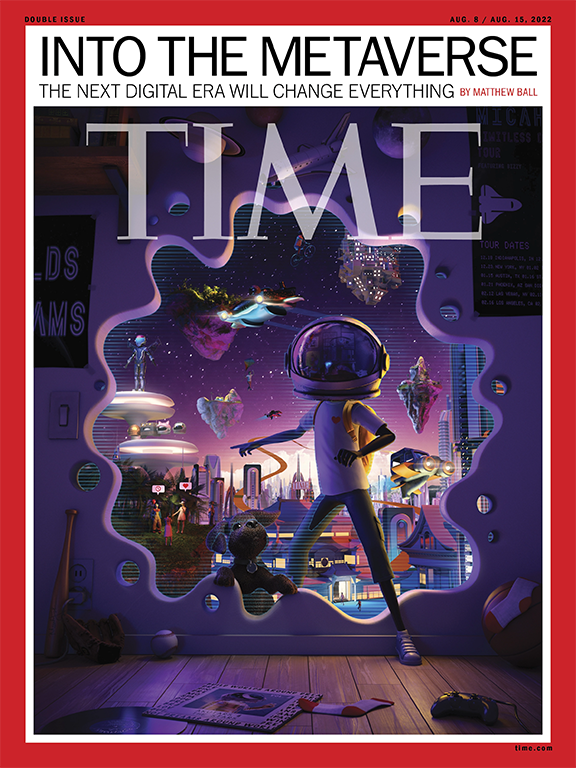
\includegraphics[width=0.5\linewidth]{time}
  \caption{Time magazine Metaverse Cover 2022}
  \label{fig:time}
\end{figure}
He \href{https://www.matthewball.vc/all/epicprimer1}{talks about Epic's Unreal engine} and identifies what he calls the Epic Flywheel for games manufacture seen in Figure \ref{fig:epicflywheel}.\par
\begin{figure}
  \centering
    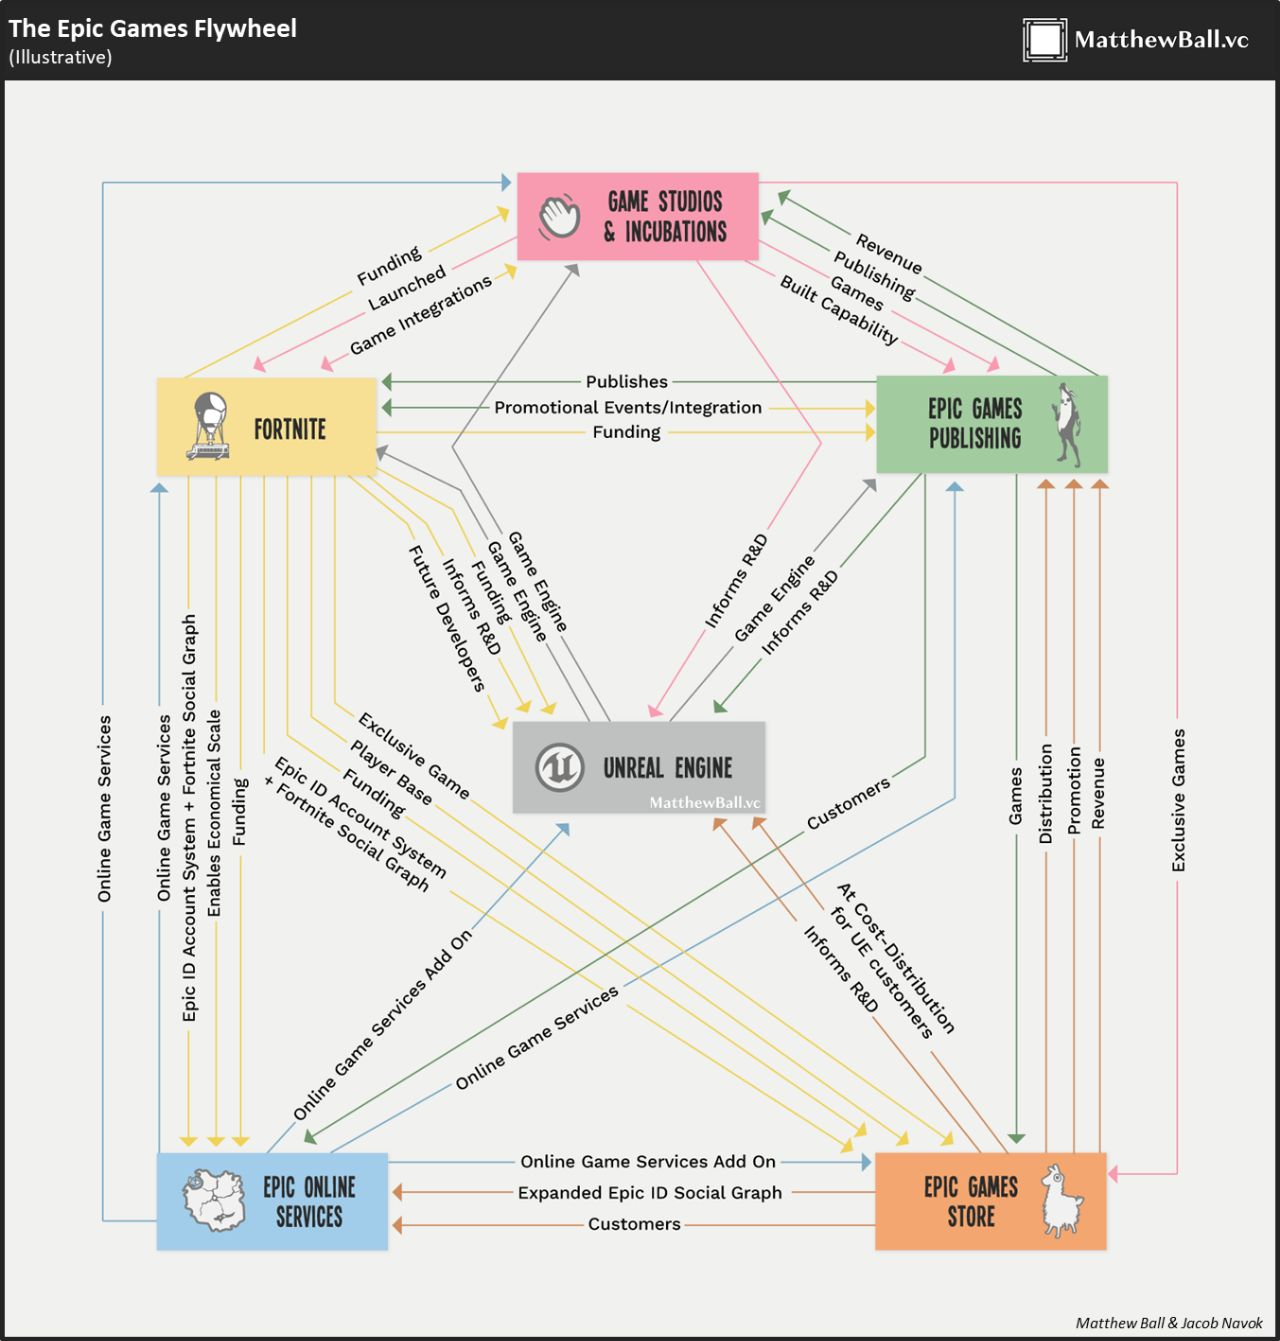
\includegraphics[width=0.7\linewidth]{epicflywheel}
  \caption{Epic games flywheel by Matthew Ball}
  \label{fig:epicflywheel}
\end{figure}
Epic is a behemoth and has made better business development decisions, and have a better technology than their main competitor Unity3D. Unity didn't make the cut for this book, though their technology is great. Their recent merger with a \href{https://www.pcgamer.com/unity-is-merging-with-a-company-who-made-a-malware-installer/}{malware manufacturer} and a history of poor data privacy have removed them from consideration at this time.
\subsection{Virtual Production}
\begin{figure}[ht]
  \centering
    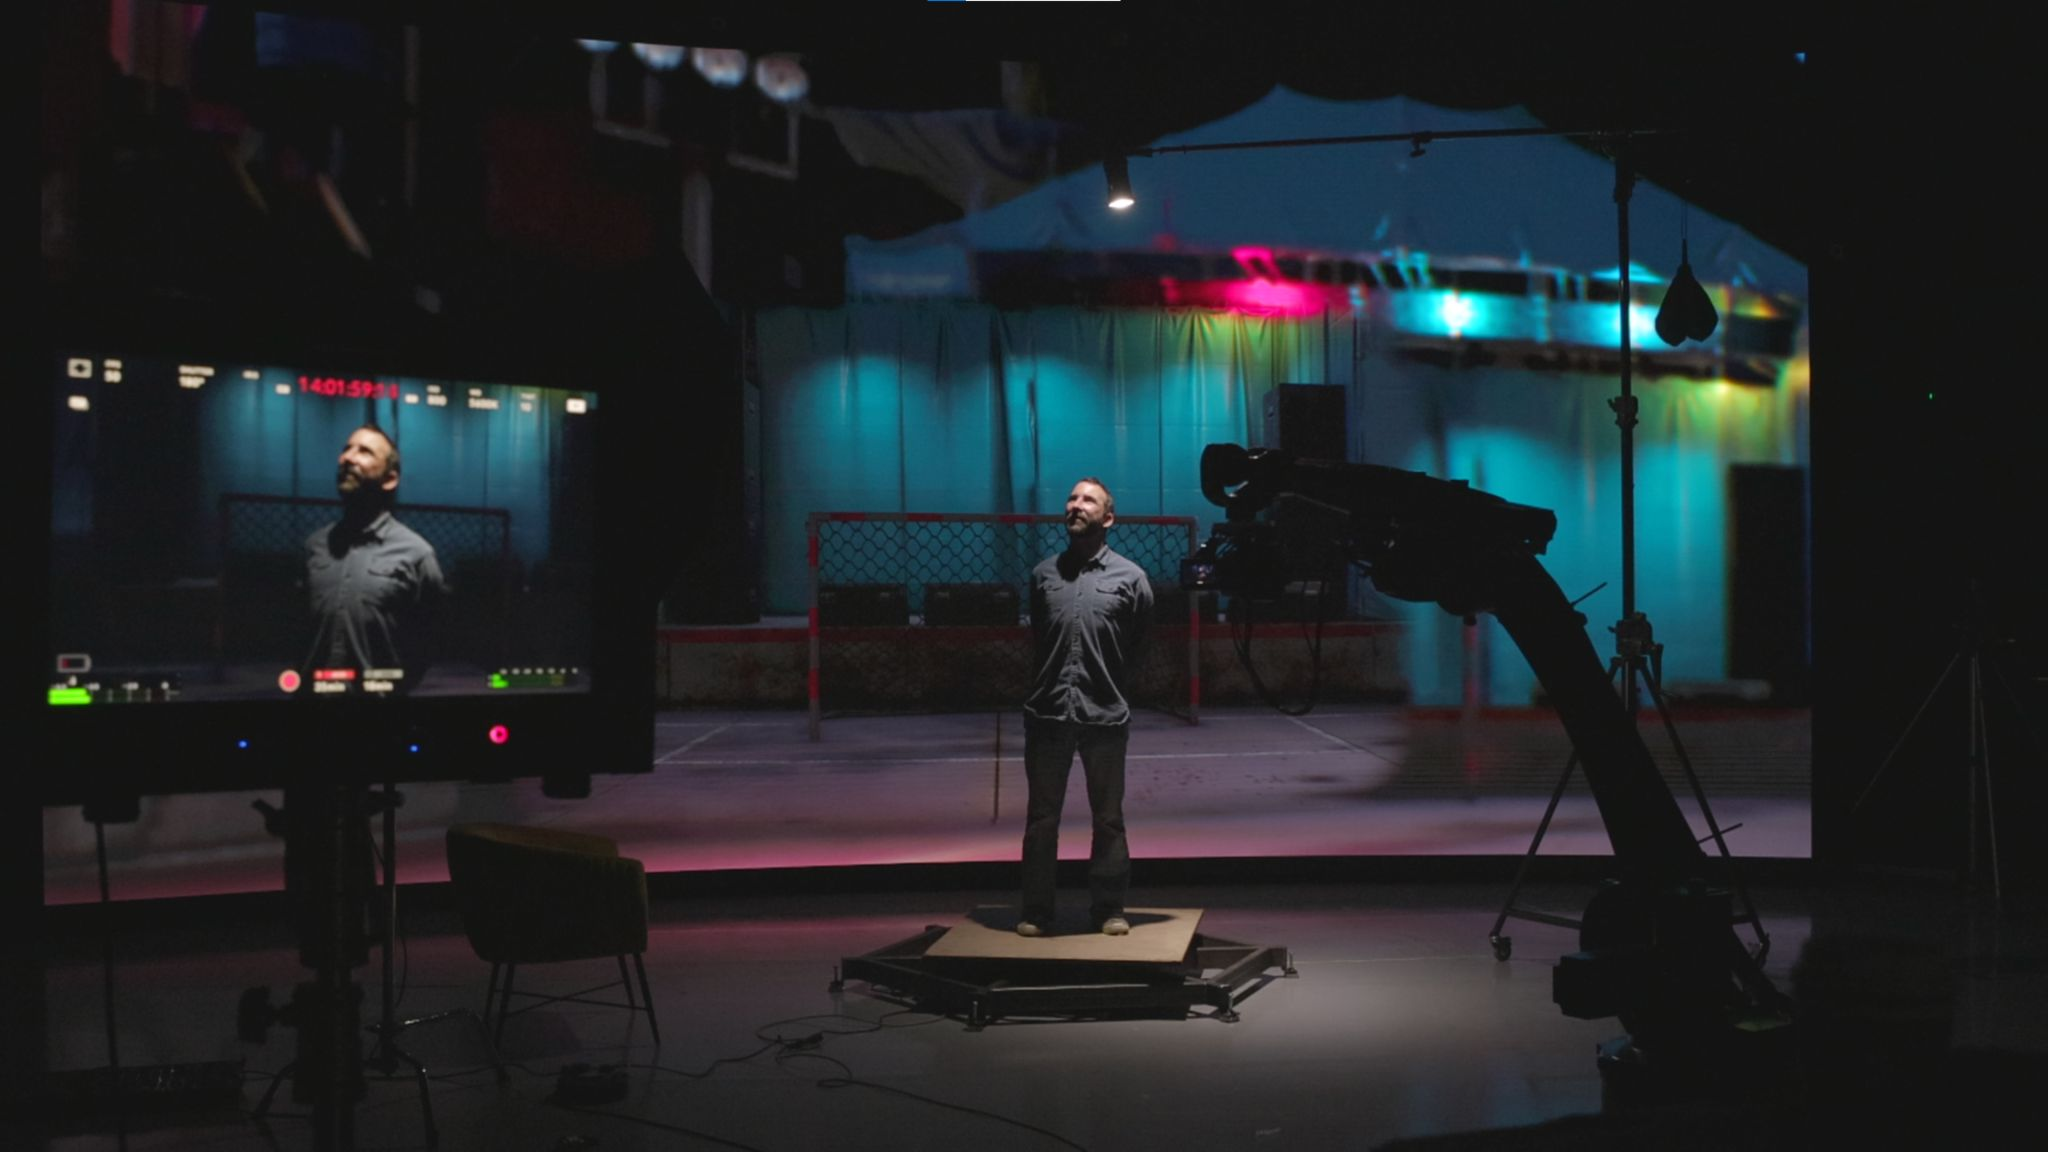
\includegraphics[width=0.7\linewidth]{pathwayrobot}
  \caption{John O'Hare (author) with a virtualproduction robot at PathwatXR.}
  \label{fig:pathwayrobot}
\end{figure}
\section{Different modalities}
\subsection{Mixed reality as a metaverse}
\input{08_MR}
\subsection{Augmented reality}
Marc Petit, general manager of Epic Games envisages a 2 watt pair of glasses, connected to a 10 watt phone, connected to a 100 watt computer on the edge. This is a device cascade problem which has not yet been solved, and is at the edge of achievable thermodynamics and latency.\par
The closest technology at this time seems to be \href{https://lumusvision.com/}{Lumus' waveguide projectors} which are light, bright and high resolution. 
\subsection{Ubiquitous displays}
This includes \href{https://skarredghost.com/2022/06/28/mojo-vision-contact-tested-eye/}{laser retinal displays}, and smart screens which are context and user aware.
\section{Risks}
Metaverse is fraught with risks, partly because it's new, and partly because of the pace of adoption. Regulation is well behind the technology, to the alarm of some academic observers \cite{rosenberg2022regulation}.
\begin{itemize}
\item Abuse; because of the real-time and spatio-temporal abuse happens less like in the current web 2 social media, and more like in the real world, but with less opportunity for repercussions. It might be that natural language processing and machine learning can help with this, but it's a tough problem. One idea might be to record the speech to text of interactions between participants, and flag to them if a ``bullying, harassment, predation threshold'' is met. This could be encrypted with the public keys of the participants and a notice sent to them that if they wished to follow up with authorities then they have the necessary attestations and proofs. This is minimally invasive and privacy preserving, and acts as a strong disincentive to repeat offence. It can also feed into a global ``web of trust'' reputation system in a `zero knowledge' way. Users who flag abuse to the reputation system can leverage the machine learning opinion without revealing what happened (though they would have the data). This would also act as a disincentive without the social stigma issues of reporting.\par
Reporting could be achieved without machine learning identification of potential problems, but there would have to be a social cost to reporting (like gossiping incessantly about others) which would erode the social score of the reporting entity. This would mitigate bot based reputation harm.
\item Miscommunication; which as we have seen in the early section of the metaverse chapter is both complex and hard to mitigate
\item Lost information
\item Distraction
\item Jitter, judder, jagginess, and interruption of flow; because the network overhead is higher than other communication media it's much more exposed to latency effects 
\item Physical harms, especially to developing brains and ocular systems
\end{itemize}
%\section{Money in metaverses}
%This is going to be a pretty big section.
%\href{Meta Pay for payments across their ecosystems}{https://www.facebook.com/zuck/posts/pfbid021Q1ZMJFWcXBvPcaqpLWgp3x5HTMD3vyVNbPB17BcuX6n1UmAKh7Kyv6dUb6oKP7Nl}
%\input{08_sidelined}
